% !TeX root = ../report.tex
% Chapter 3: Methodology
\chapter{การออกแบบและวิธีการดำเนินงาน}
\thaijustify{
  ในบทที่ 3 จะกล่าวถึงการสำรวจและวิเคราะห์ความต้องการของระบบ การออกแบบระบบ สถาปัตยกรรมโดยภาพรวม การออกแบบส่วนต่อประสานผู้ใช้ และการพัฒนาระบบที่ดำเนินการในภาคการศึกษาที่ 1
}
\section{การสำรวจและวิเคราะห์ความต้องการของระบบ}
\subsection{การสัมภาษณ์ผู้มีส่วนได้ส่วนเสีย}
\thaijustify{
  \todo{กลุ่มที่สัมภาษณ์ จำนวนผู้ให้สัมภาษณ์ วิธีการ และข้อค้นพบหลัก}
}
\subsection{ข้อค้นพบและความต้องการที่ได้จากการสัมภาษณ์}
\thaijustify{
  \todo{สรุป pain point และความต้องการที่นำมากำหนด requirement}
}

\section{ความต้องการของระบบ}
\subsection{Functional Requirements}
\thaijustify{
  \todo{Functional requirements แยกตามส่วนของระบบ}
}
\subsection{Non-Functional Requirements}
\thaijustify{
  \todo{Non-functional requirements เช่น ความปลอดภัย, PDPA, ประสิทธิภาพ, การใช้งาน}
}

\section{การออกแบบระบบ (System Design)}
\begin{samepage}
  \subsection{Use Case Diagram}
  \thaijustify{
    แผนภาพกรณีการใช้งาน (Use case diagram) แสดงความสัมพันธ์ระหว่างผู้ใช้งานแต่ละบทบาทกับฟังก์ชันของแพลตฟอร์ม โดยแบ่งออกเป็น 4 ส่วน ได้แก่ ส่วน Authentication, ส่วนสร้าง two-alternative UI, ส่วนทดสอบการใช้งานและรับความเห็น, และส่วนสร้างรายงาน
  }
  \subsubsection{Authentication}
  \begin{figure}[H]
    \centering
    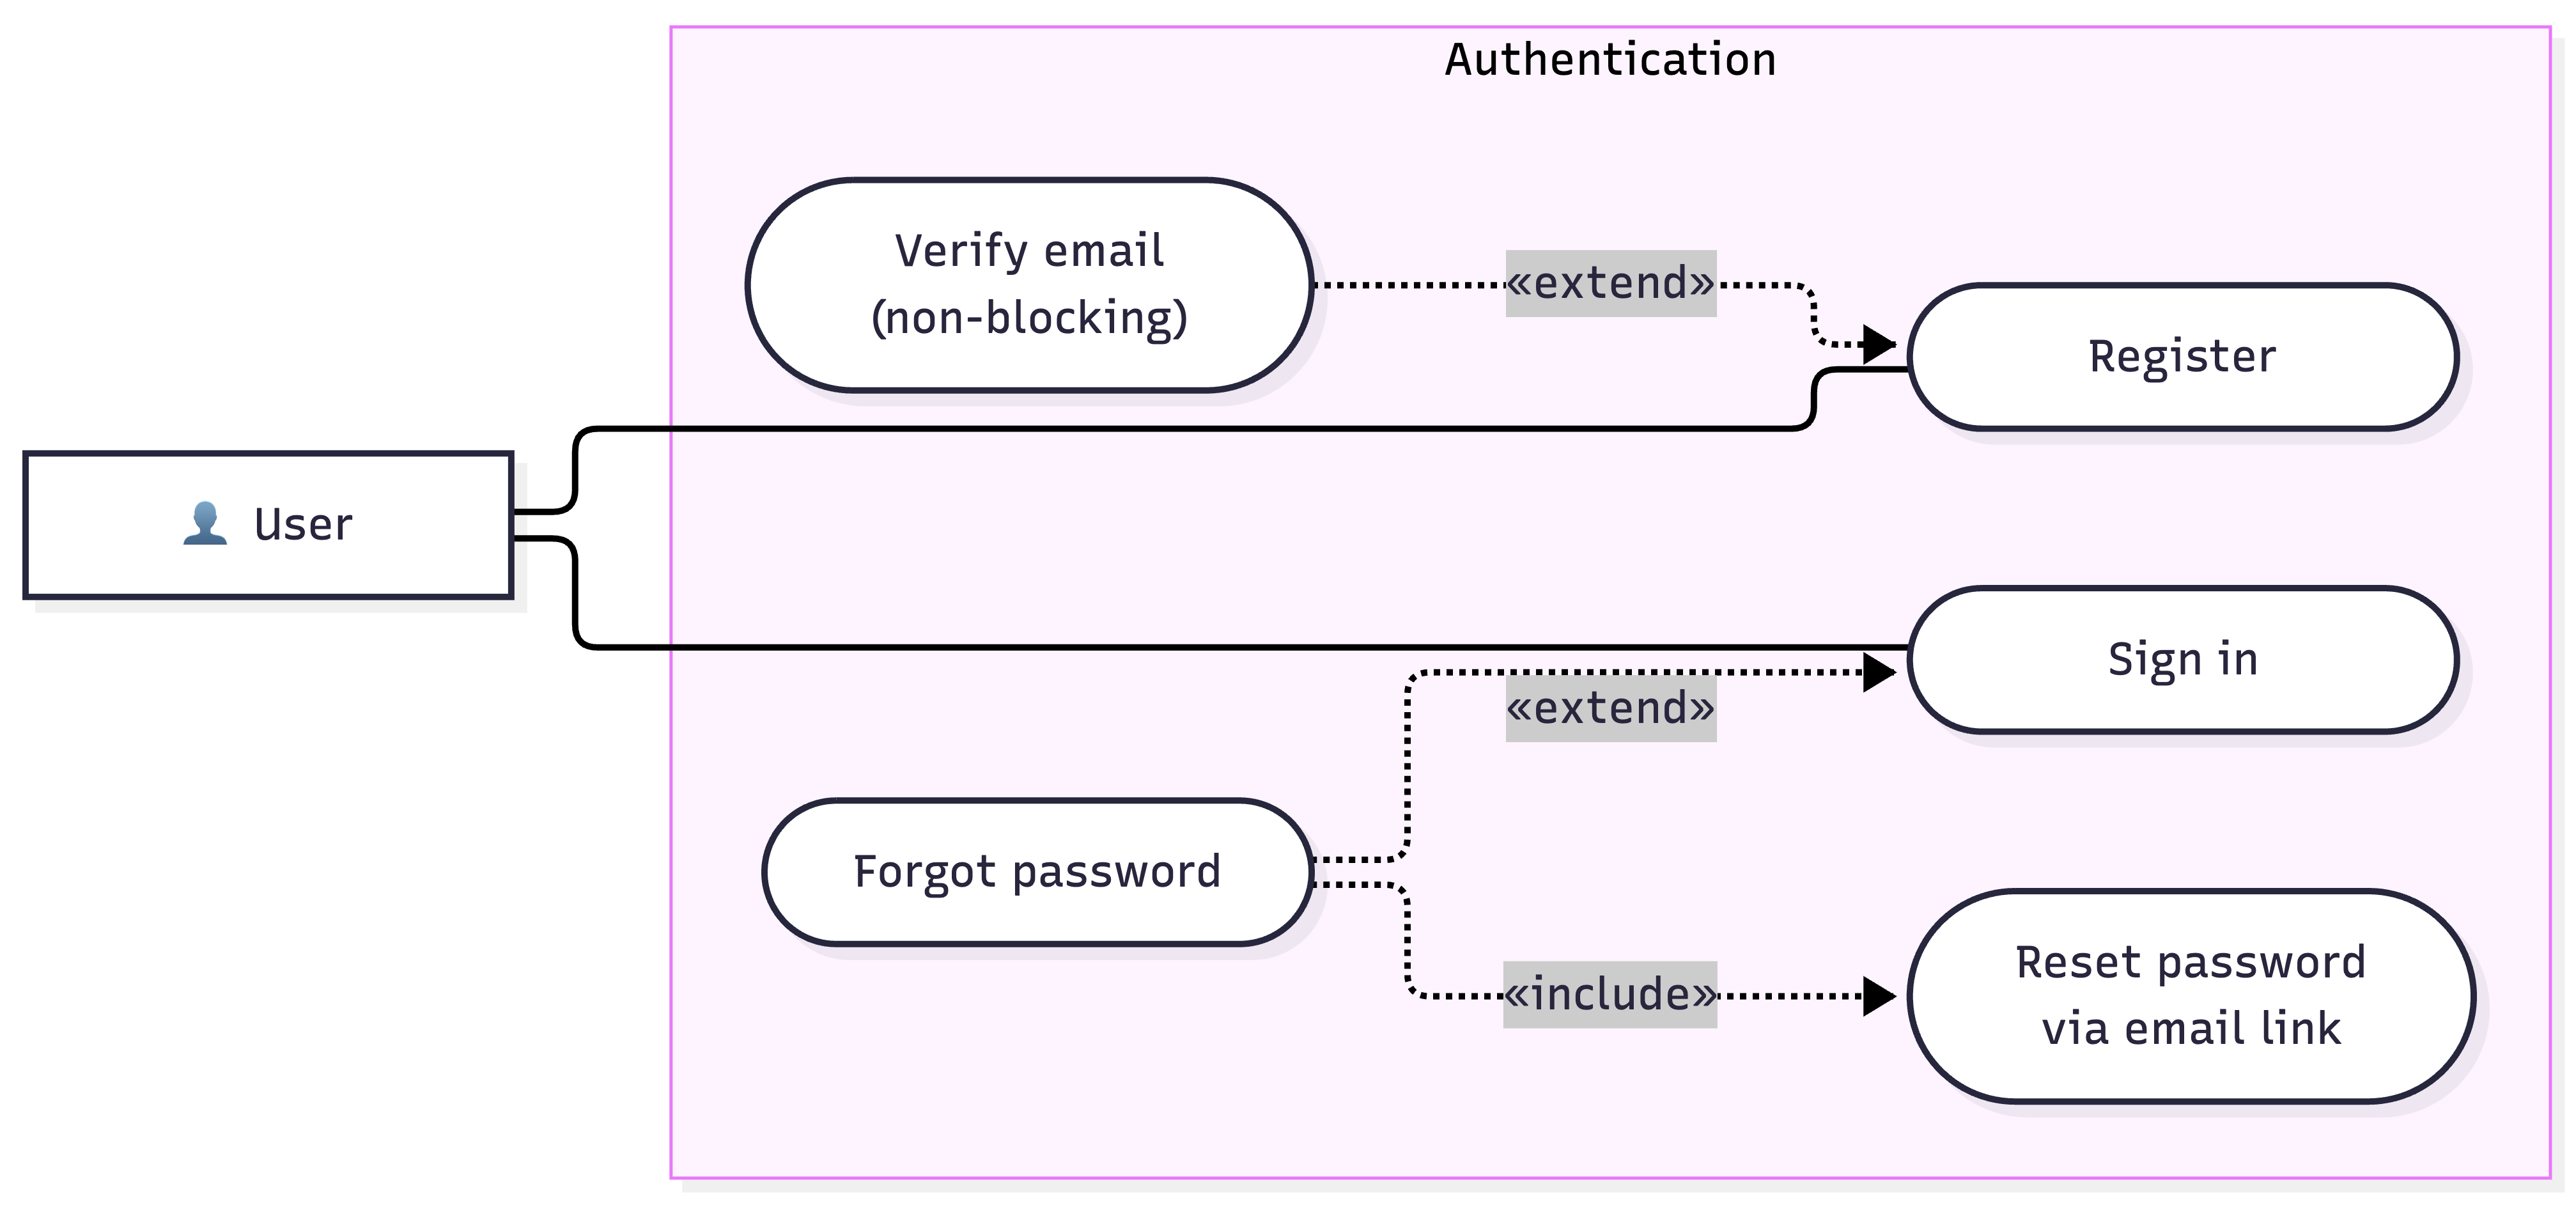
\includegraphics[
      width=0.6\textheight,
      height=\linewidth,
      keepaspectratio,
      origin=c
    ]{figures/ch3-methodology/UC-1.png}
    \caption{Use case diagram for authentication}
    \label{fig:UC-1}
    \thaijustify{ภาพแสดง Use Case ของระบบ Authentication โดยผู้ใช้สามารถสมัครสมาชิก เข้าสู่ระบบ และกู้คืนรหัสผ่านได้ โดยการยืนยันอีเมลเป็นขั้นตอนเสริมหลังการสมัคร และการรีเซ็ตรหัสผ่านดำเนินการผ่านลิงก์ที่ส่งทางอีเมล}
  \end{figure}
  \subsubsection{Designer: Project setup \& UI Generation}
  \begin{figure}[H]
    \centering
    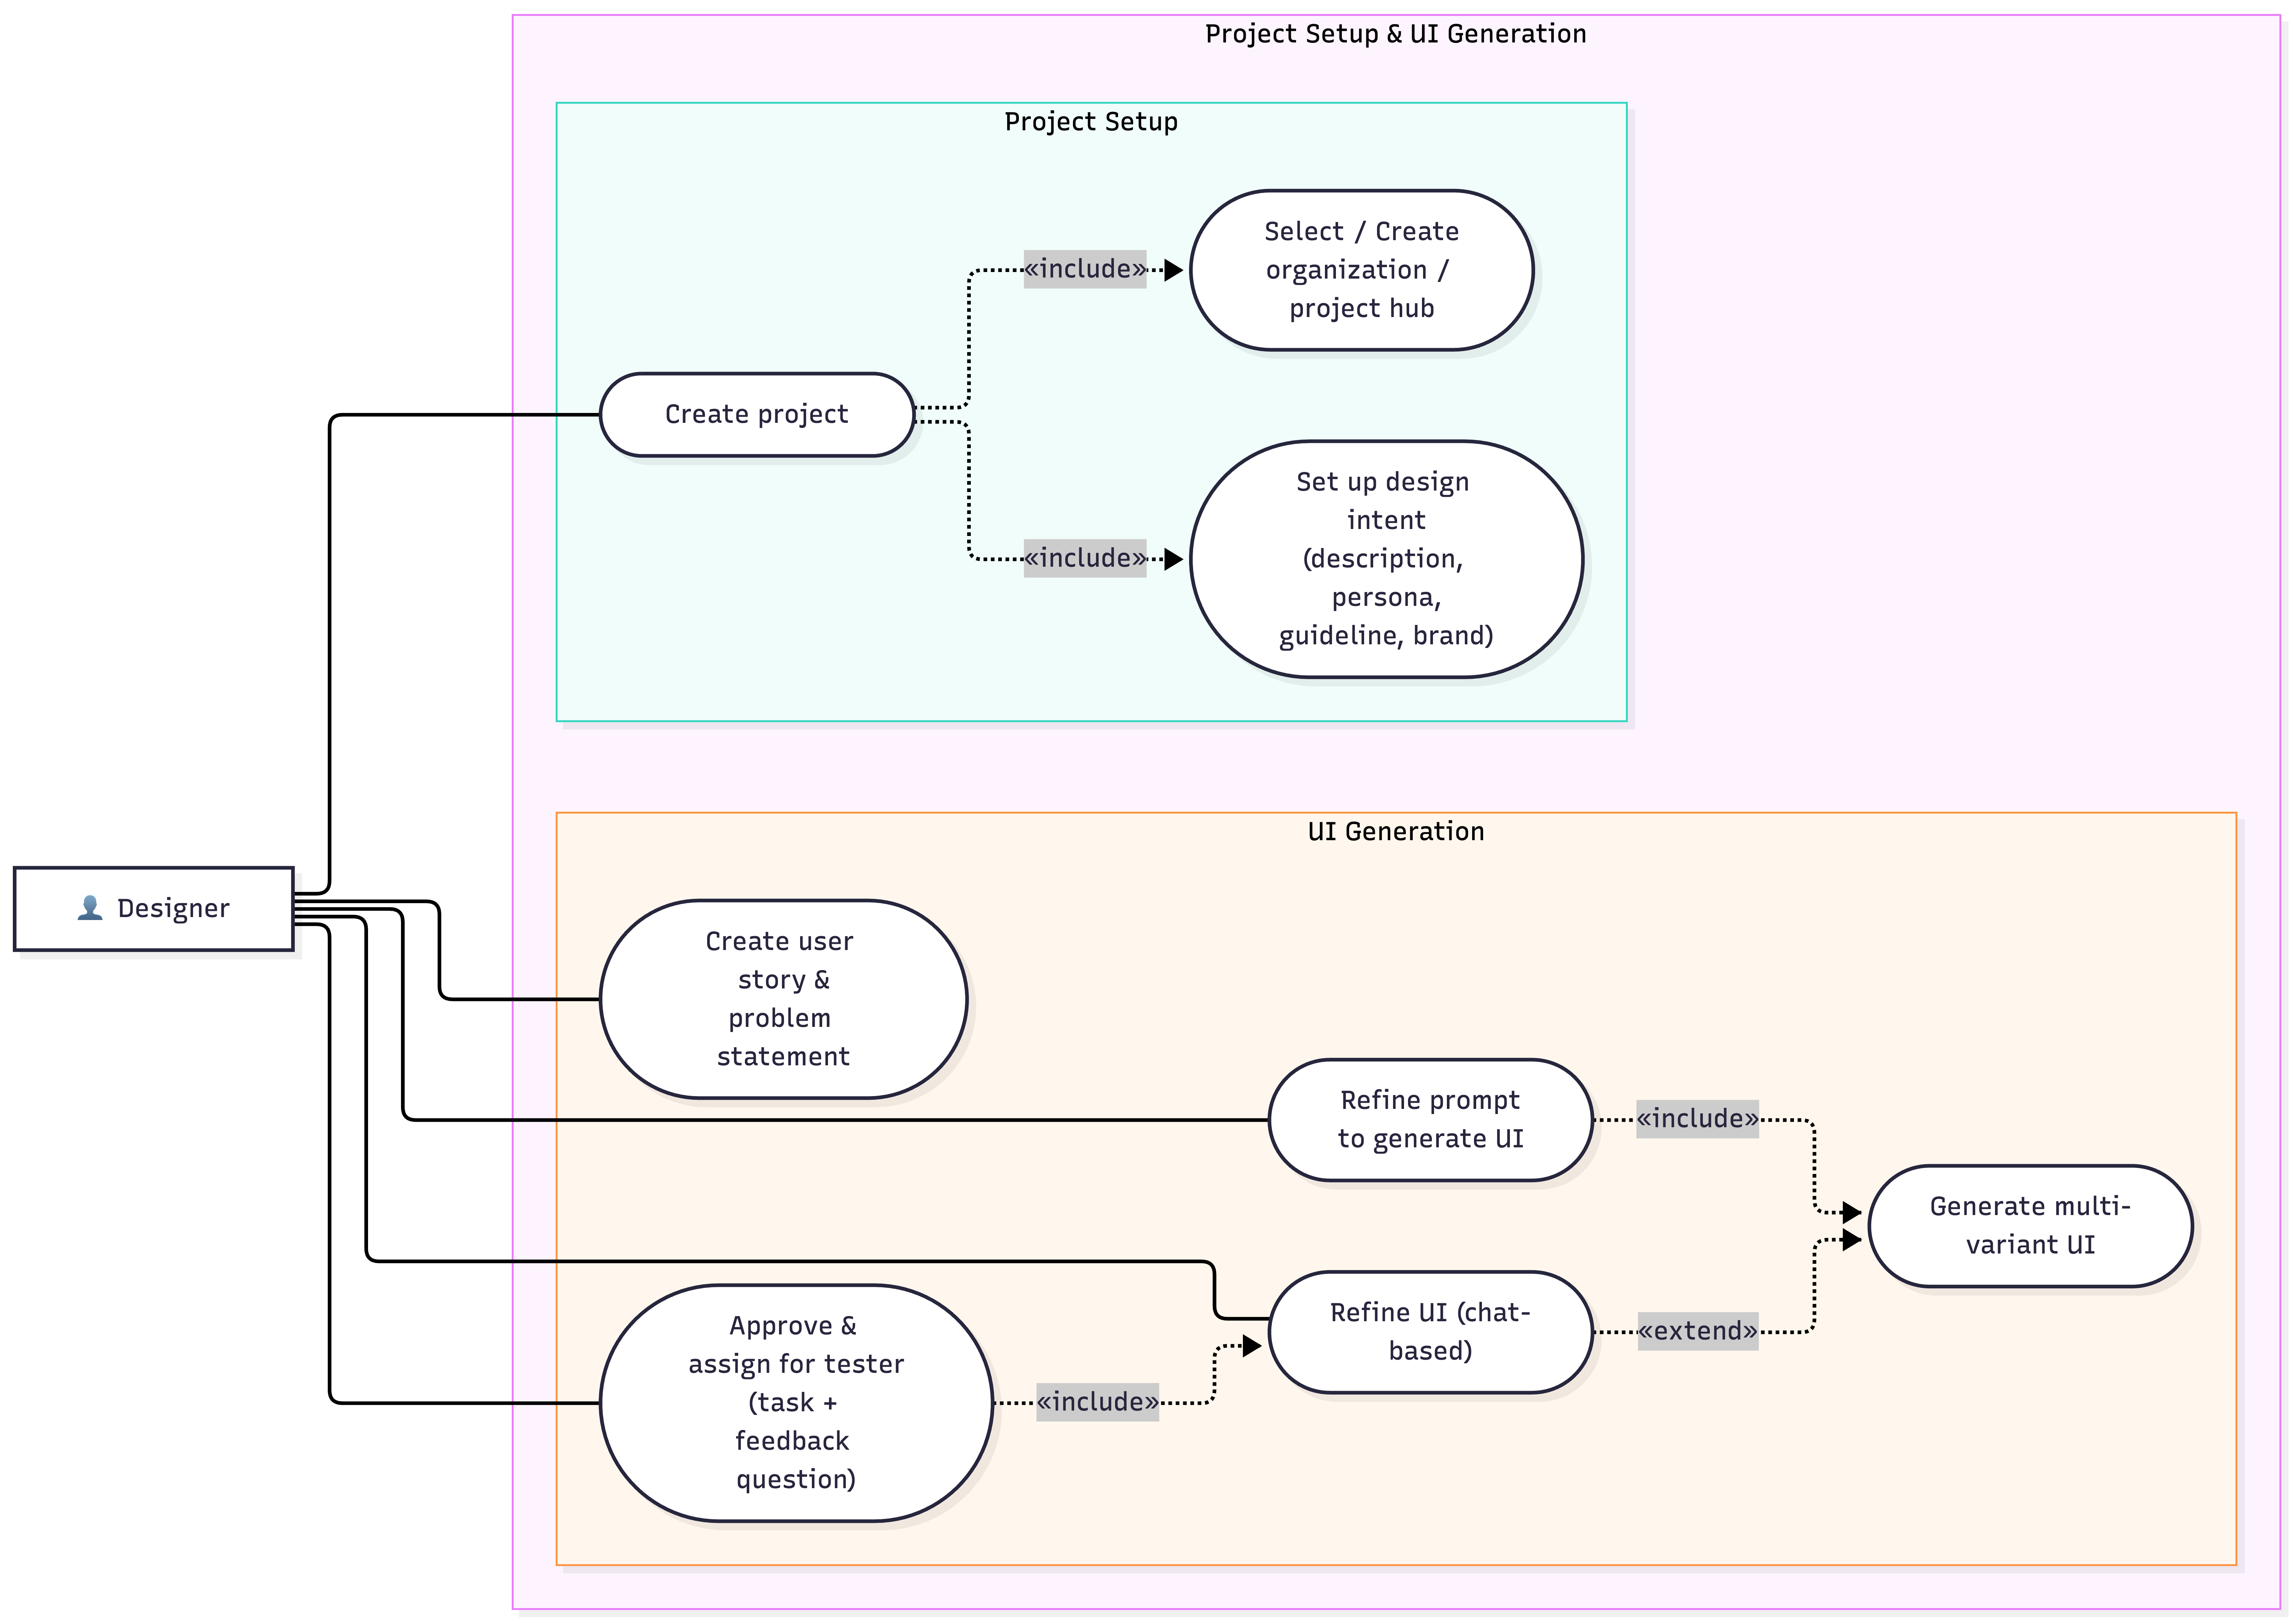
\includegraphics[
      width=0.6\textheight,
      height=\linewidth,
      keepaspectratio,
      origin=c
    ]{figures/ch3-methodology/UC-2.png}
    \caption{Use case diagram for Project setup and UI Generation}
    \label{fig:UC-2}
    \thaijustify{ภาพแสดง Use Case ของกระบวนการจัดเตรียมโครงการและสร้าง UI โดย Designer สามารถสร้างโครงการ กำหนด Design Intent สร้างและปรับแต่ง Prompt เพื่อสร้าง UI หลายรูปแบบ รวมถึงปรับแก้ UI และอนุมัติเพื่อส่งให้ผู้ทดสอบประเมิน}
  \end{figure}
  \subsubsection{Designer and Tester: Testing session and Feedback analysis}
  \begin{figure}[H]
    \centering
    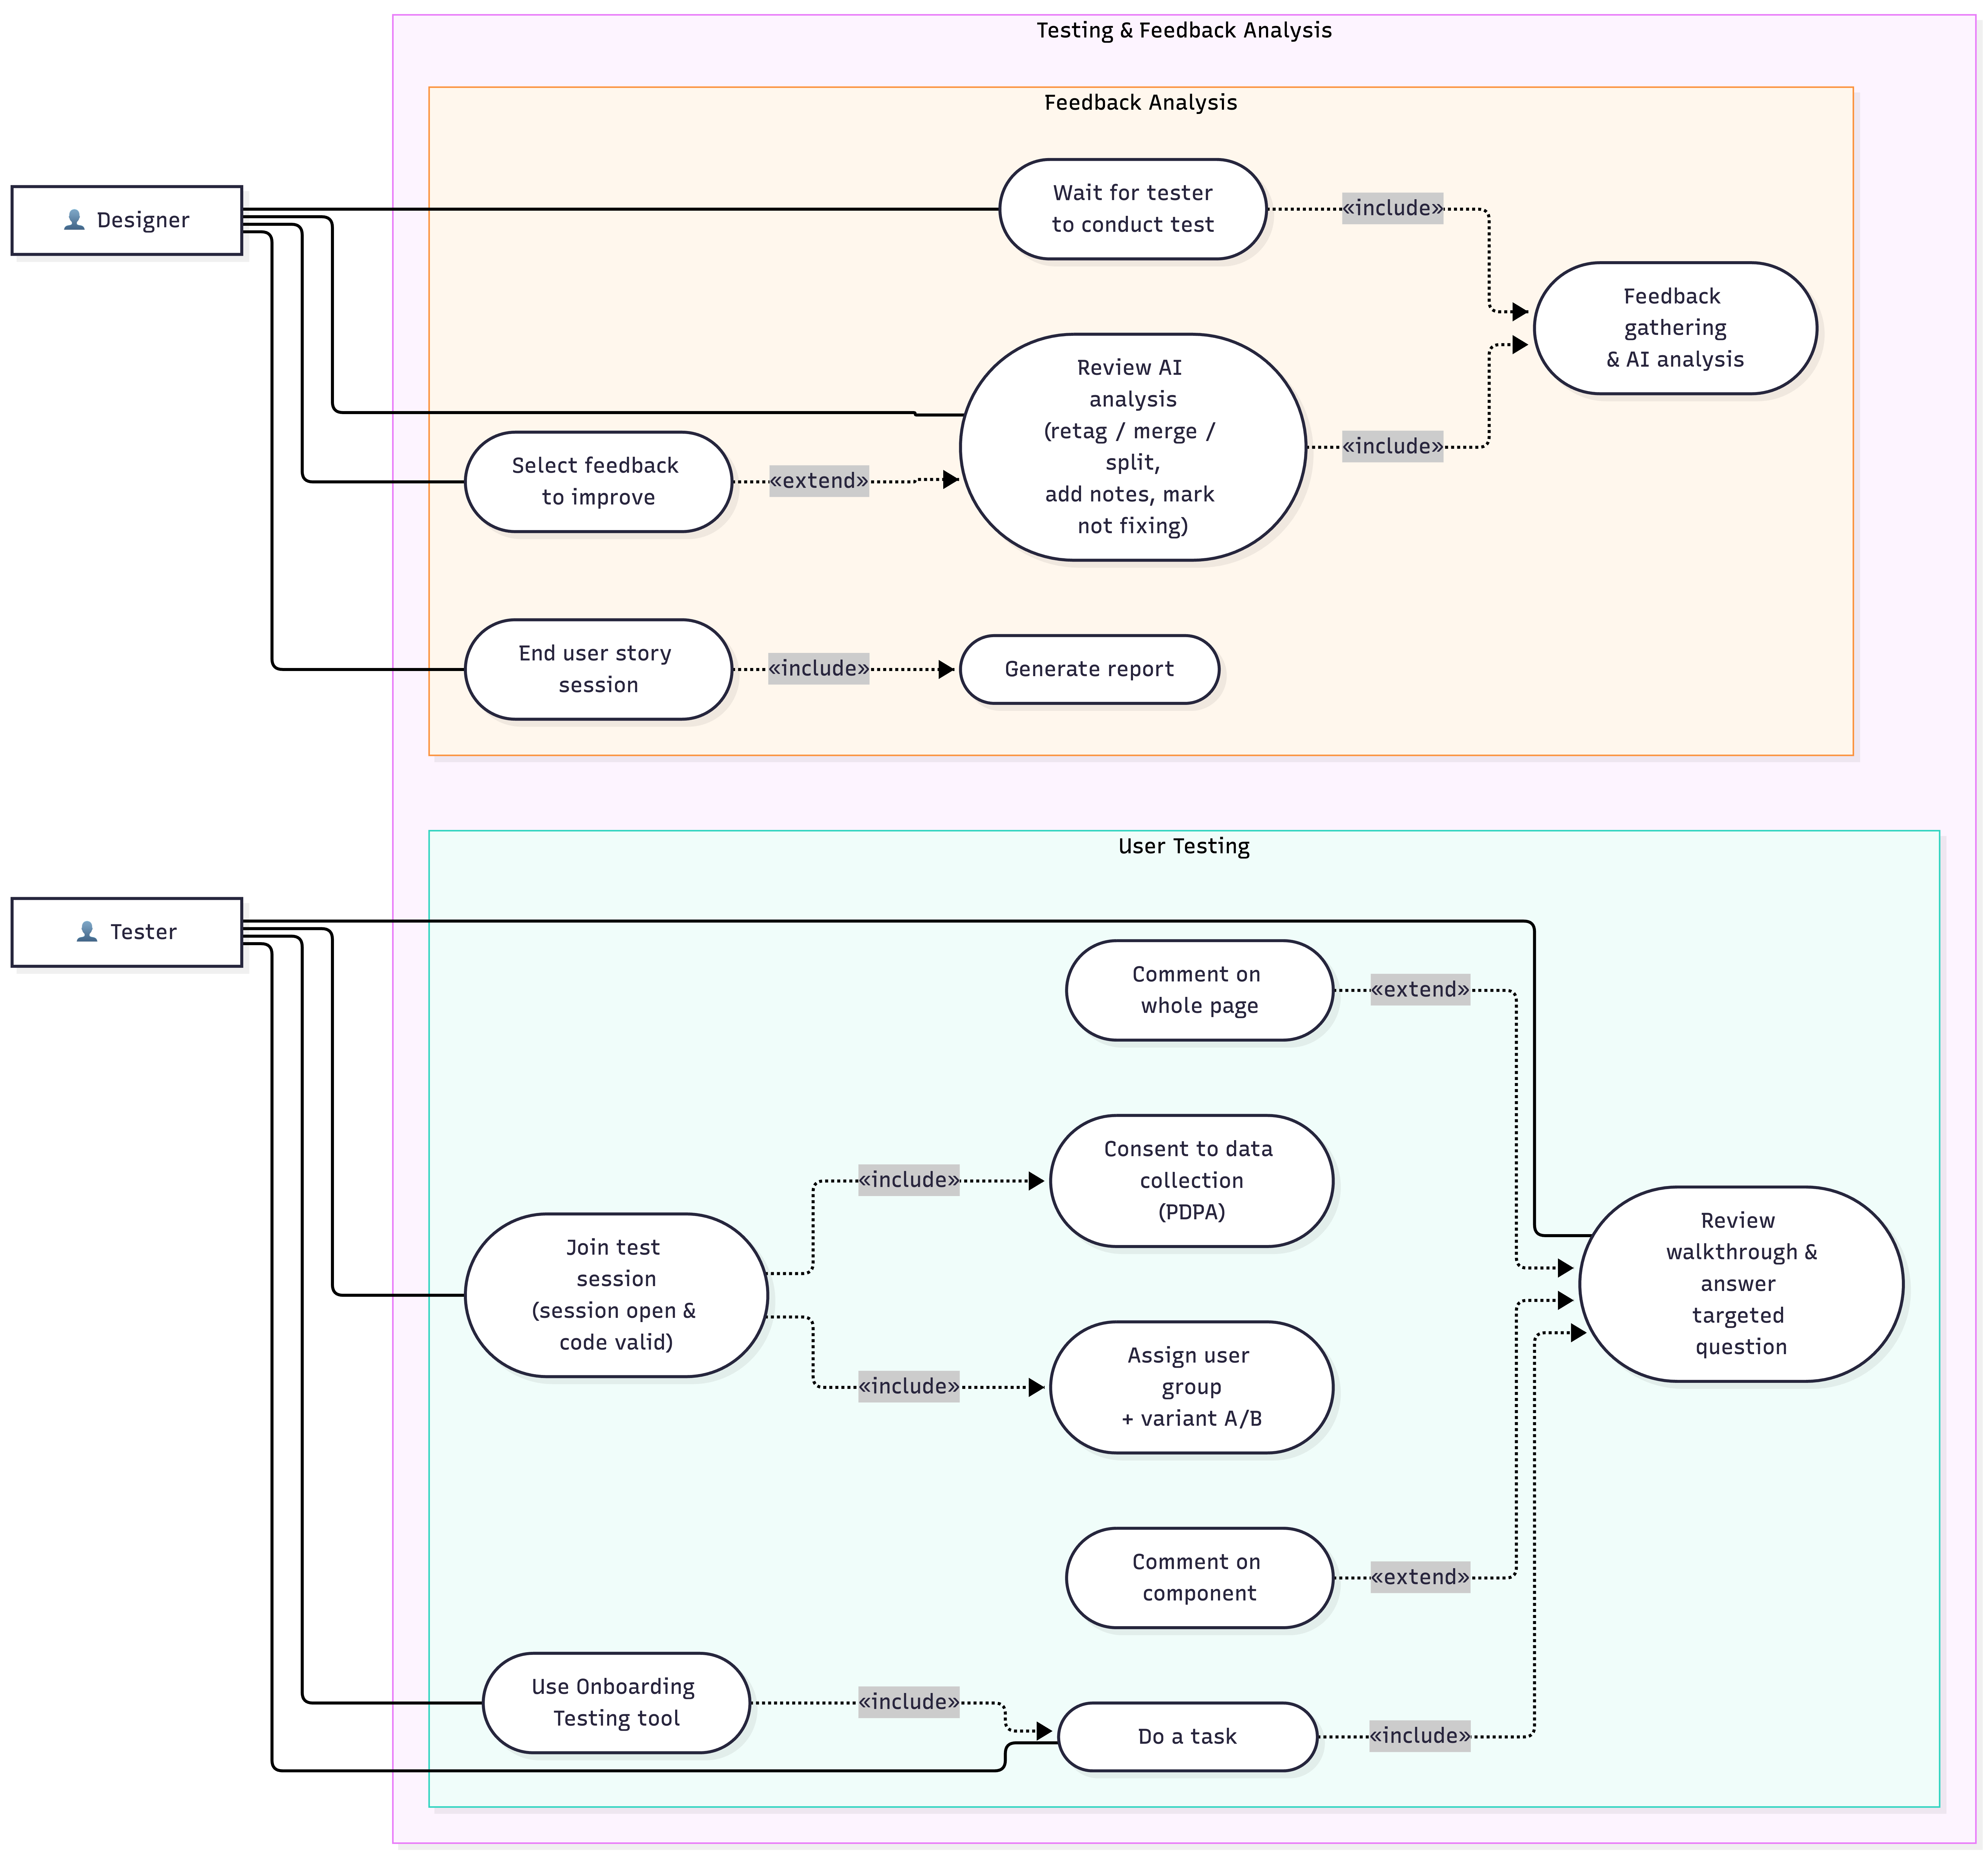
\includegraphics[
      width=0.6\textheight,
      height=\linewidth,
      keepaspectratio,
      origin=c
    ]{figures/ch3-methodology/UC-3.png}
    \caption{Use case diagram for Testing session and Feedback analysis}
    \label{fig:UC-3}
    \thaijustify{ภาพแสดง Use Case ของกระบวนการทดสอบและวิเคราะห์ Feedback โดย Tester เข้าร่วมการทดสอบ ทำภารกิจ และให้ความคิดเห็น ขณะที่ Designer รวบรวมและตรวจสอบผลการทดสอบ วิเคราะห์ Feedback ด้วย AI และเลือกประเด็นเพื่อนำไปปรับปรุงส่วนต่อประสานผู้ใช้}
  \end{figure}
  \subsubsection{Client, Developer, and Project Manager: Project view and Report}
  \begin{figure}[H]
    \centering
    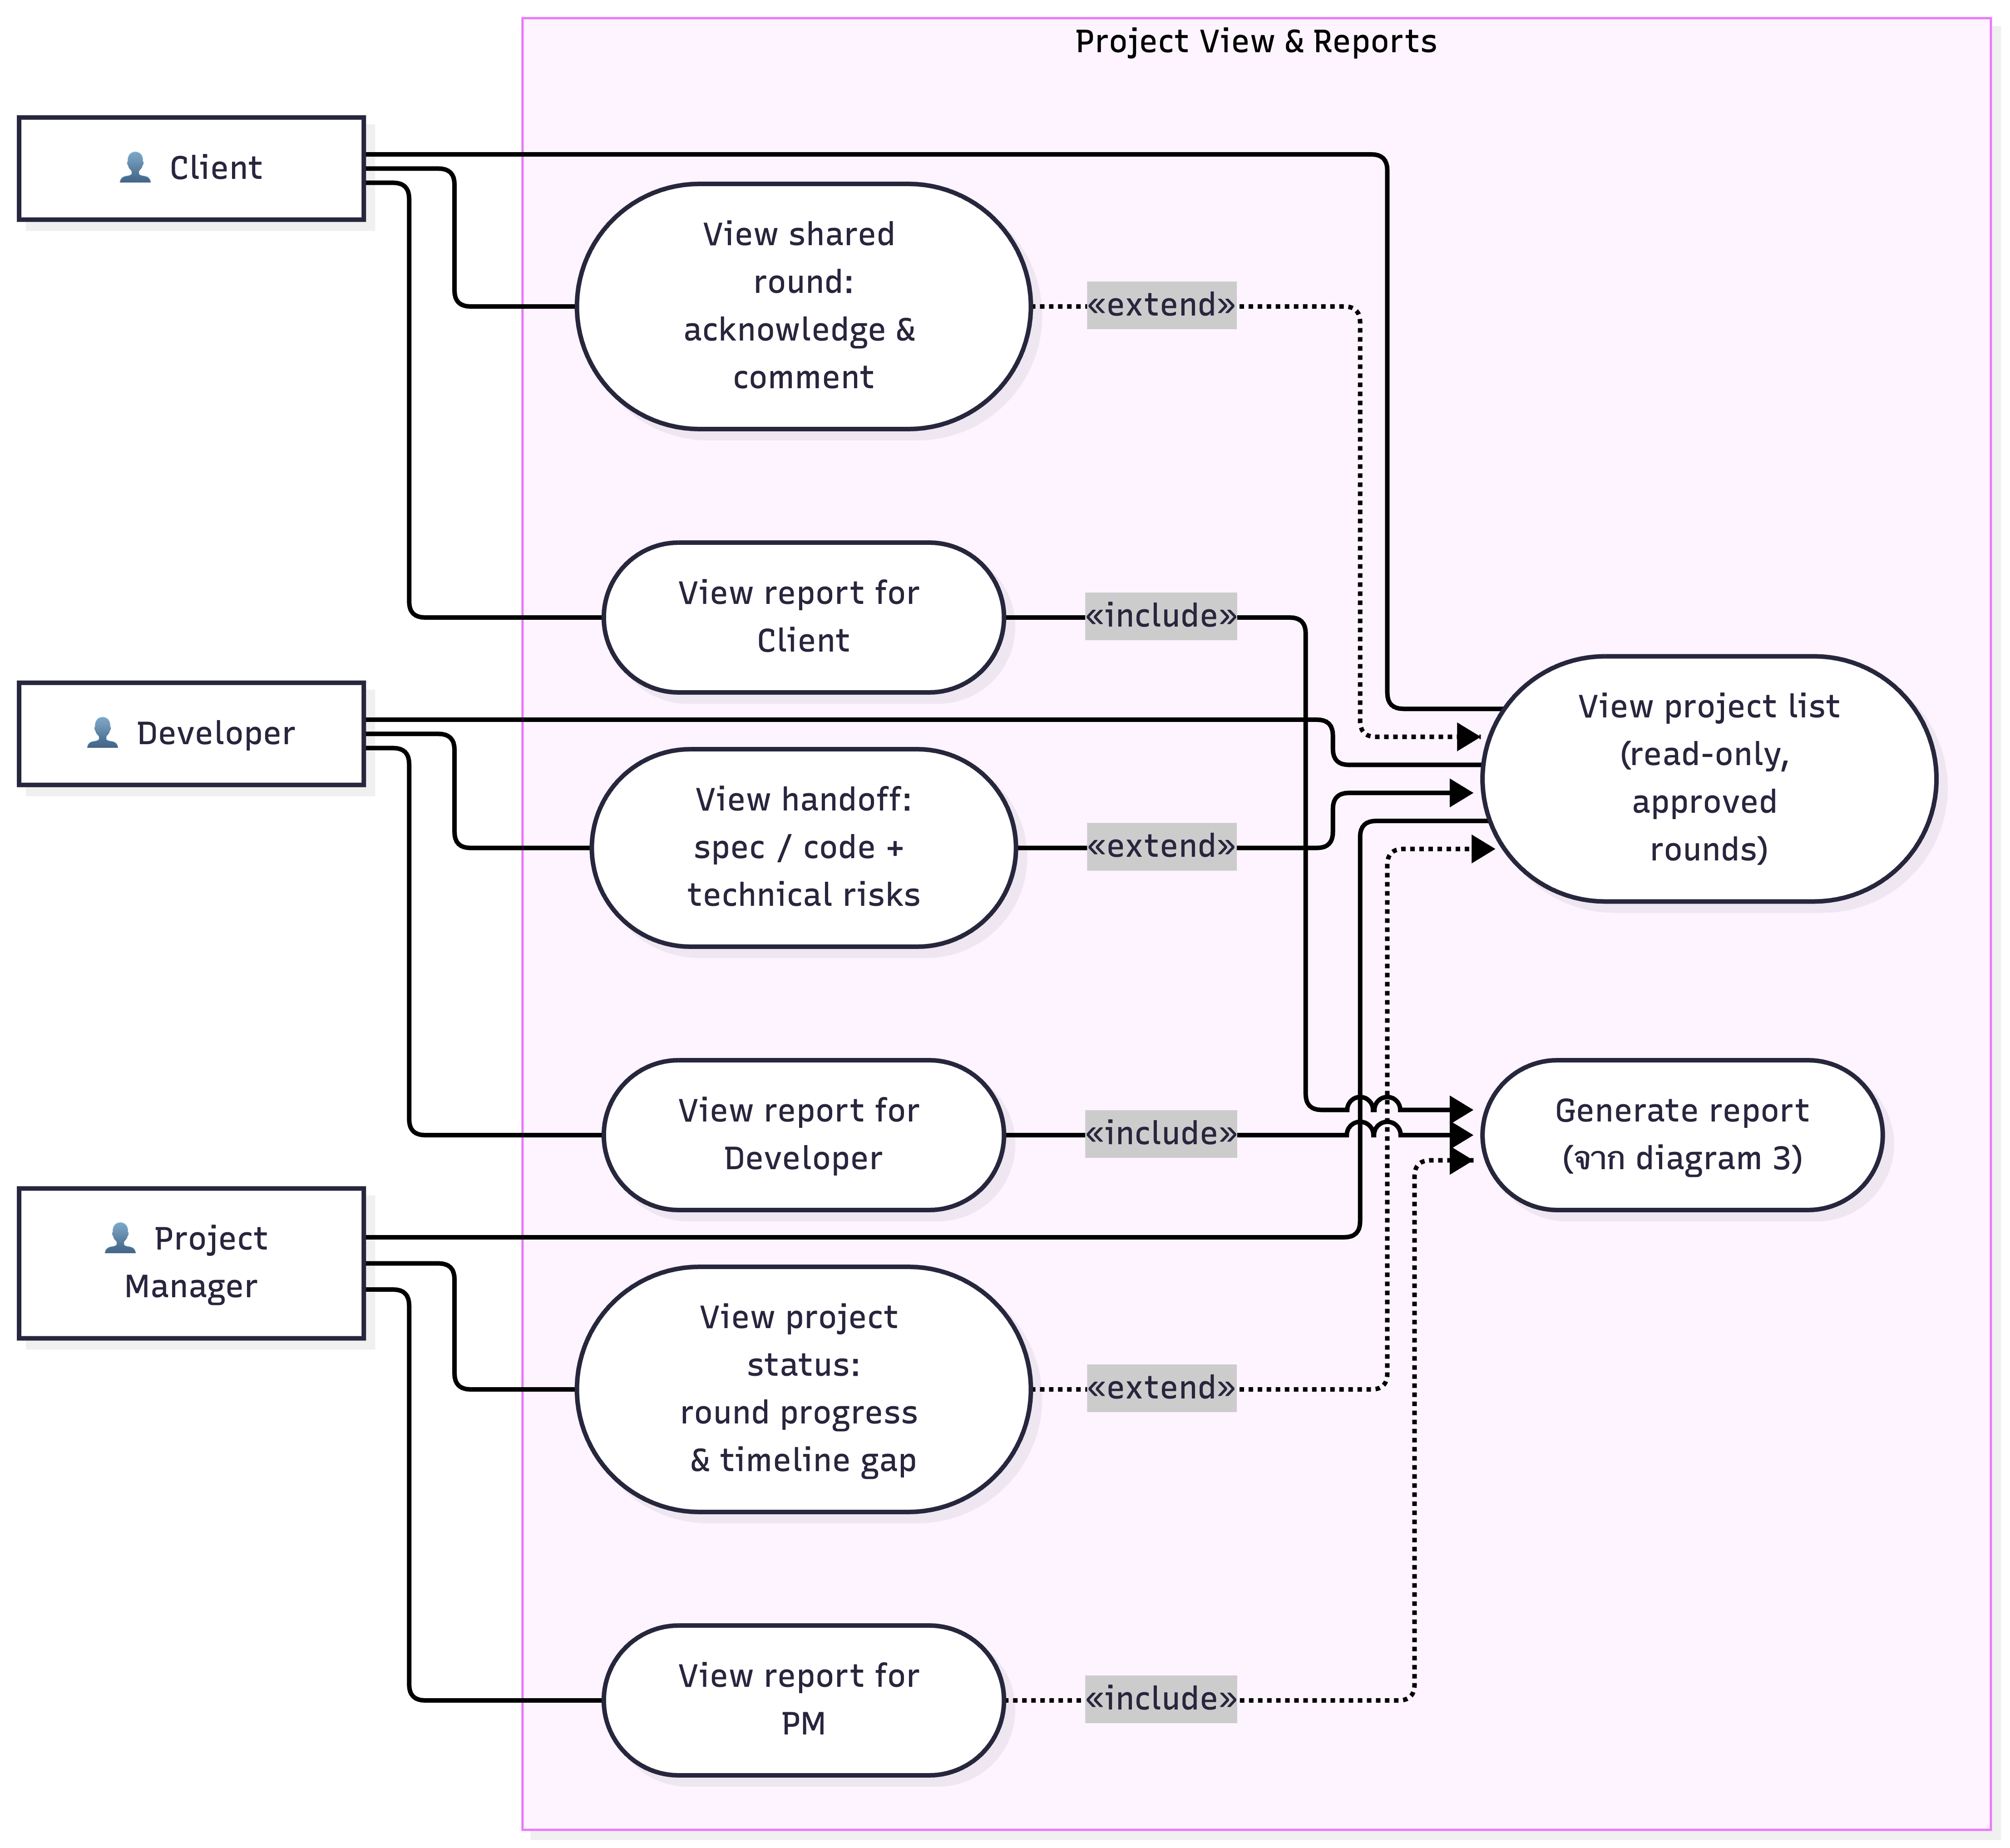
\includegraphics[
      width=0.6\textheight,
      height=\linewidth,
      keepaspectratio,
      origin=c
    ]{figures/ch3-methodology/UC-4.png}
    \caption{Use case diagram for Project view and Report}
    \label{fig:UC-4}
    \thaijustify{
      ภาพแสดง Use Case ของการดูโครงการและรายงาน โดย ผู้ใช้งาน, นักพัฒนา และ ผู้ดูแลโครงการ สามารถดูข้อมูลโครงการที่ได้รับอนุมัติและข้อมูลที่เกี่ยวข้องตามบทบาท รวมถึงดูรายงานที่สร้างจากผลการทดสอบและ Feedback
    }
  \end{figure}
\end{samepage}

\subsection{Sequence Diagram}
\thaijustify{
  \todo{Sequence diagram ของกระบวนการหลัก เช่น การสร้าง two-alternative UI และการทดสอบ}
}

\subsection{ER Diagram}\label{sec:er-diagram}
\thaijustify{
  ฐานข้อมูลของแพลตฟอร์มใช้ PostgreSQL และกำหนดโครงสร้างผ่าน Prisma schema ประกอบด้วย 34 ตารางและ 25 ชนิดข้อมูลแบบ enum เพื่อให้อ่านง่าย จึงแบ่ง ER diagram ออกเป็นสี่กลุ่มตามส่วนของระบบ (รูปที่~\ref{fig:er-workspace-project} ถึง~\ref{fig:er-analysis-report}) ในแต่ละตารางแสดง primary key (PK), foreign key (FK) และคอลัมน์หลักบางส่วน ส่วนตารางสีเทาเป็นตารางจากกลุ่มอื่นที่แสดงไว้เพื่อให้เห็นความสัมพันธ์
}
\thaijustify{
  \textbf{ผู้ใช้ workspace และโปรเจกต์ (รูปที่~\ref{fig:er-workspace-project}):} ผู้ใช้ (User) เข้าสู่ระบบผ่านบัญชีภายนอก (Account) และได้รับ refresh token ที่เก็บเป็นค่า hash แยกตามกลุ่มของการเข้าสู่ระบบ (familyId) ผู้ใช้สร้างหรือได้รับเชิญเข้า workspace โดยมีบทบาท ADMIN หรือ MEMBER (WorkspaceMember) ภายใน workspace มีหลายโปรเจกต์ (Project) และสมาชิกแต่ละคนมีบทบาทในโปรเจกต์ (ProjectMember) ได้แก่ Designer, Project Manager, Client และ Developer แต่ละโปรเจกต์มีความต้องการทางการออกแบบ (DesignIntent) หนึ่งชุด มี persona ได้หลายรายการ (UserPersona) และมีบันทึกกิจกรรม (AuditLog) สำหรับตรวจสอบย้อนหลัง
}
\thaijustify{
  \textbf{การออกแบบและการสร้าง UI ด้วย AI (รูปที่~\ref{fig:er-design-generation}):} โปรเจกต์มี user story (UserStory) ที่นักออกแบบเขียนเองหรือให้ AI ร่าง (StoryGeneration) แต่ละรอบการออกแบบ (DesignRound) อ้างอิง user story หนึ่งเรื่อง และอ้างอิงรอบก่อนหน้าได้ (parentRoundId) เมื่อสั่งสร้าง UI ระบบสร้างงาน (GenerationJob) ที่เก็บ prompt และจำนวน variant ไว้ ผลลัพธ์คือ UI variant (UIVariant) ซึ่งเก็บ HTML และผลการตรวจการเข้าถึง เมื่อนักออกแบบปรับแก้ variant ระบบสร้าง variant ใหม่ที่อ้างอิงฉบับเดิม (parentVariantId) จึงย้อนดูประวัติแต่ละเวอร์ชันได้
}
\thaijustify{
  \textbf{เซสชันการทดสอบ (รูปที่~\ref{fig:er-testing}):} เซสชันการทดสอบ (TestSession) ผูกกับรอบการออกแบบหนึ่งรอบ และเลือก variant ที่ใช้ทดสอบผ่านตาราง SessionVariant ผู้เข้าร่วมทดสอบ (SessionParticipant) ได้รับลิงก์เชิญที่เก็บเป็นค่า hash และต้องให้ความยินยอมตาม PDPA ก่อนเริ่ม ซึ่งบันทึกไว้ใน ConsentRecord พร้อมเวอร์ชันของข้อความที่ยินยอม ระหว่างทำภารกิจ (TestTask) ระบบบันทึกการทำภารกิจแต่ละครั้ง (TaskRun) พฤติกรรมการใช้งาน (InteractionEvent) และข้อเสนอแนะ (Feedback) ซึ่งระบุได้ว่าเป็นความเห็นต่อ component หรือต่อทั้งหน้าจอ
}
\thaijustify{
  \textbf{การวิเคราะห์ข้อเสนอแนะและรายงาน (รูปที่~\ref{fig:er-analysis-report}):} ผลการวิเคราะห์ข้อเสนอแนะด้วย AI เก็บใน FeedbackAnalysis และแยกเป็นประเด็น (FeedbackTheme) ที่เชื่อมกับข้อเสนอแนะต้นทางผ่าน ThemeFeedback นักออกแบบรวม แยก หรือตัดสินใจไม่แก้ไขประเด็นได้ ทุกการตัดสินใจถูกบันทึกใน DesignDecision และประเด็นที่เลือกไปปรับปรุงเชื่อมกับรอบการออกแบบถัดไปผ่าน RoundFeedbackLink ทำให้สืบย้อนได้ว่าการเปลี่ยนแปลงแต่ละครั้งมาจากข้อเสนอแนะใด ผู้มีส่วนได้ส่วนเสียแสดงความเห็นและรับทราบรอบที่อนุมัติแล้วได้ (RoundComment, RoundAcknowledgement) และระบบสร้างรายงาน (Report) แยกตามบทบาท
}

\begin{figure}[p]
  \centering
  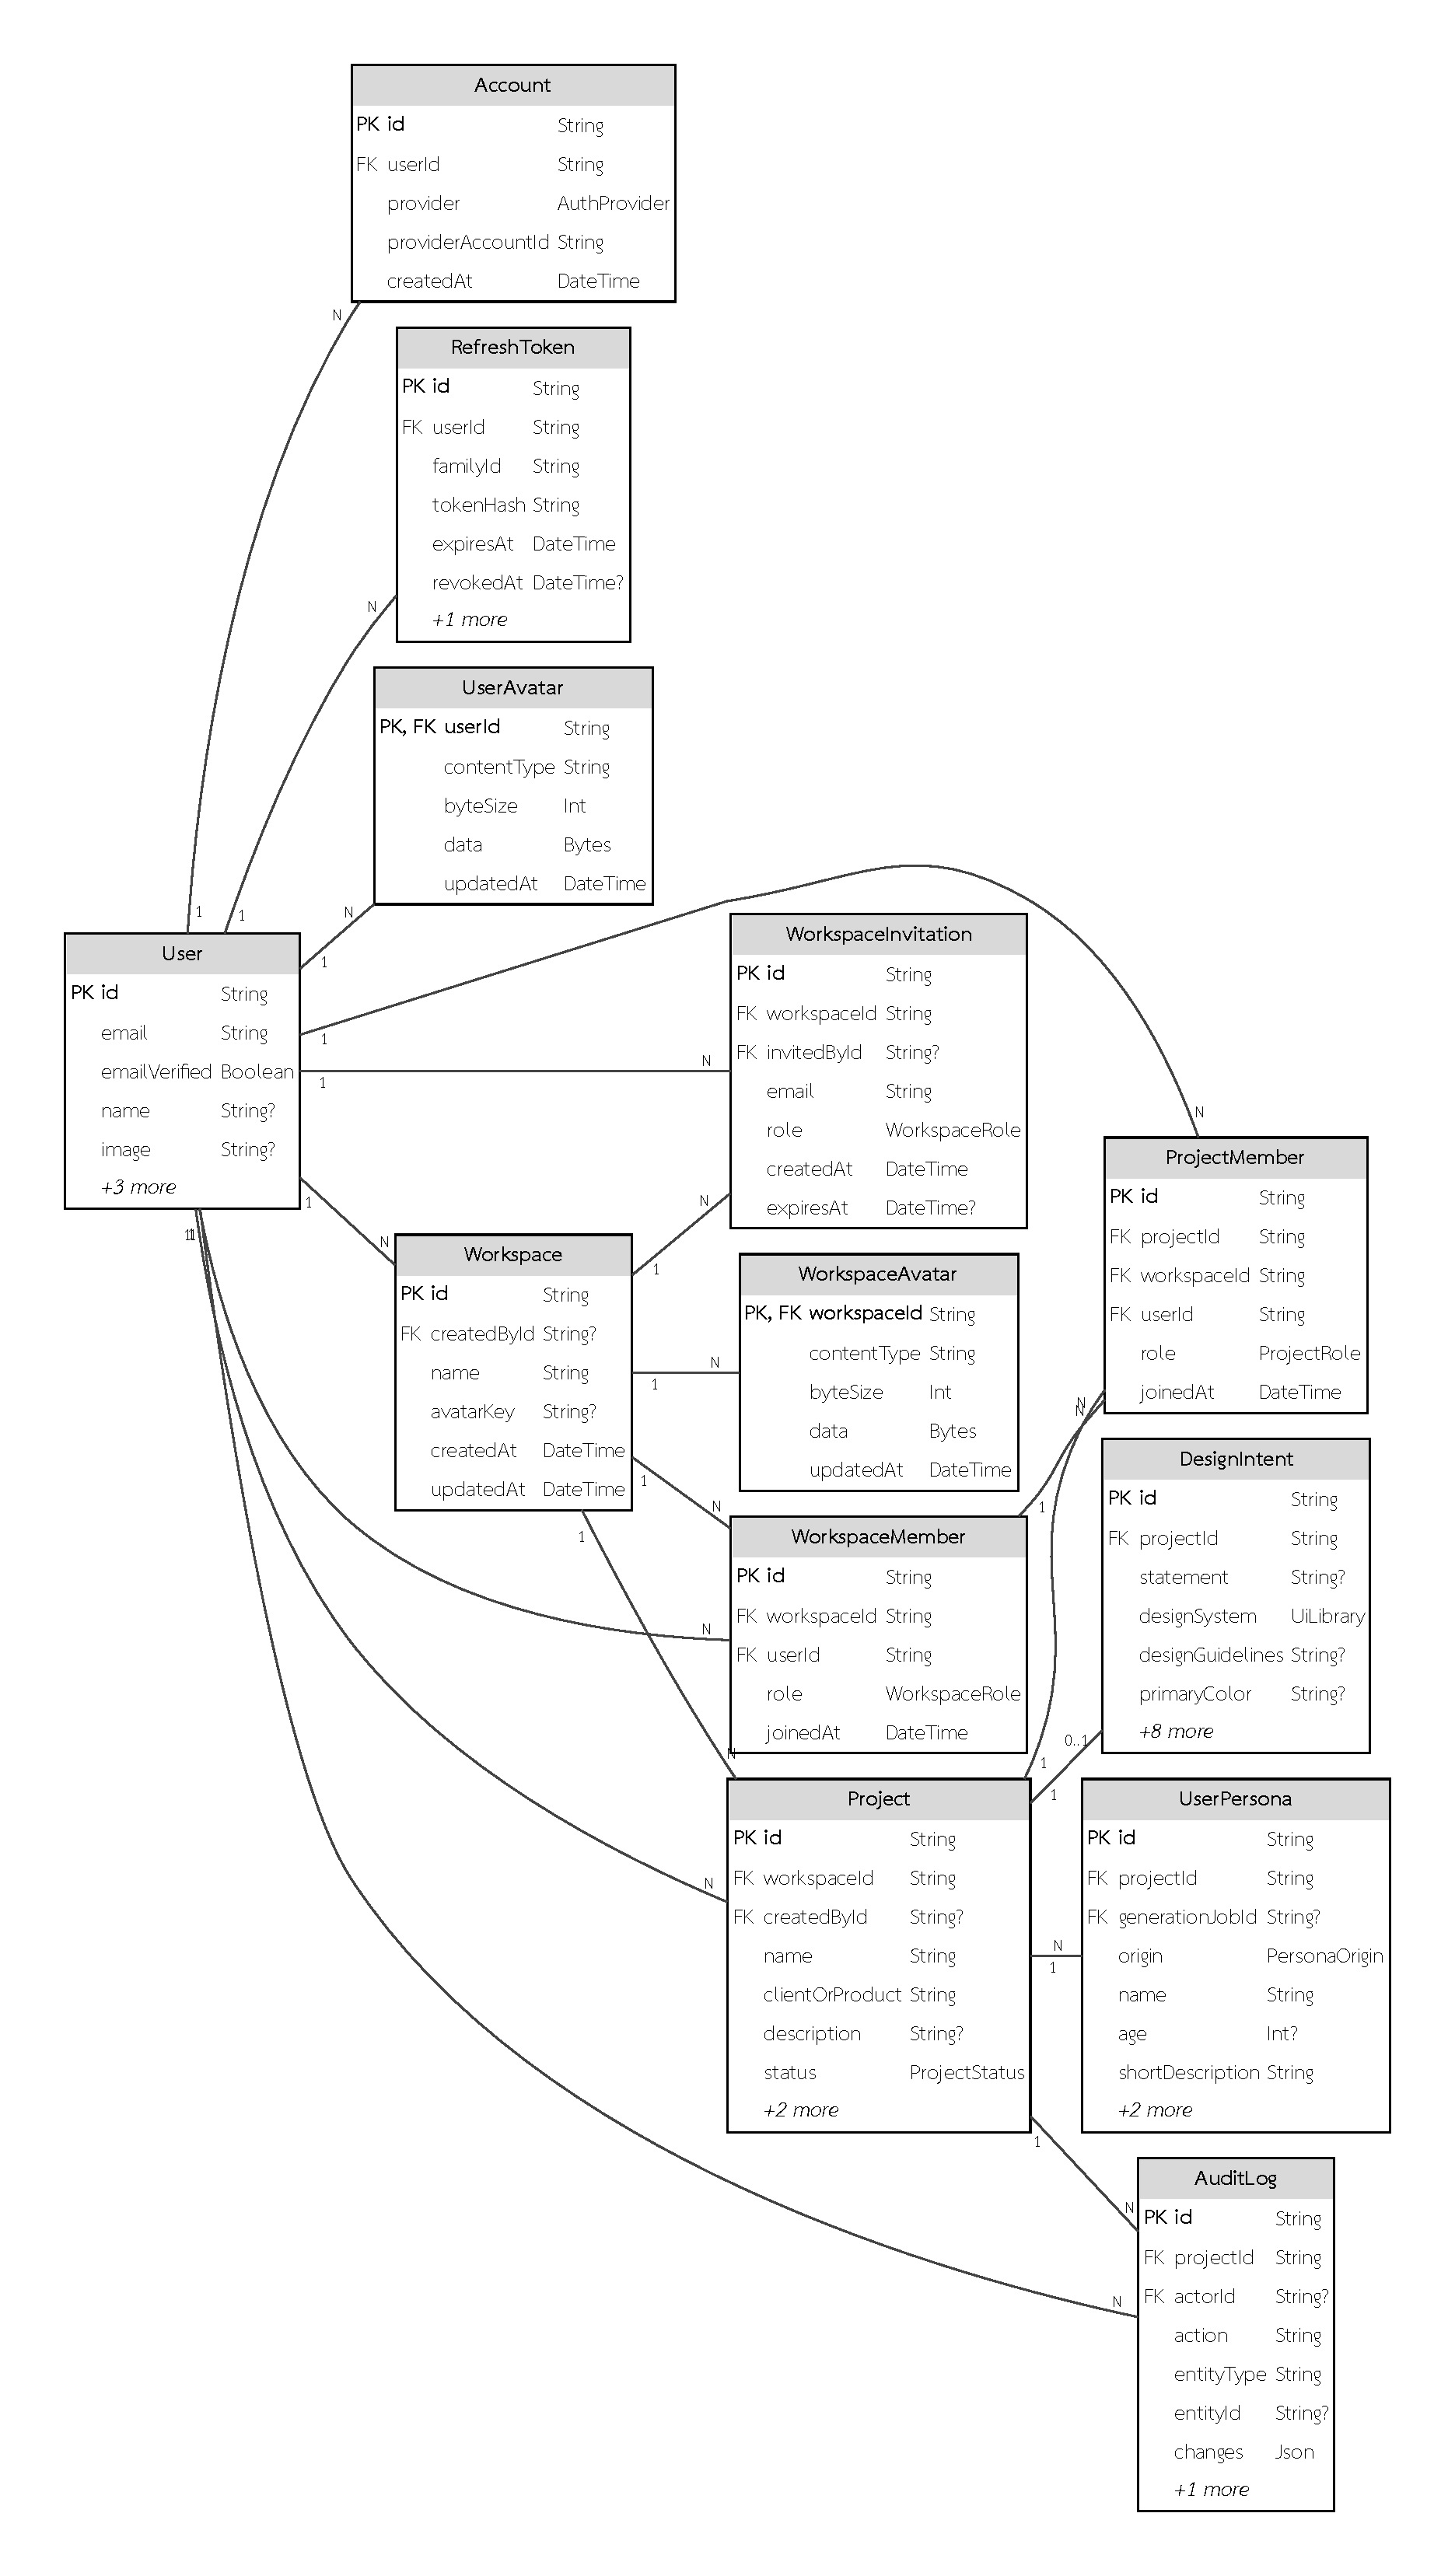
\includegraphics[width=\linewidth,height=0.88\textheight,keepaspectratio]{figures/ch3-methodology/er-workspace-project.pdf}
  \caption{ER diagram ส่วนผู้ใช้ workspace และโปรเจกต์}
  \label{fig:er-workspace-project}
\end{figure}
\begin{figure}[p]
  \centering
  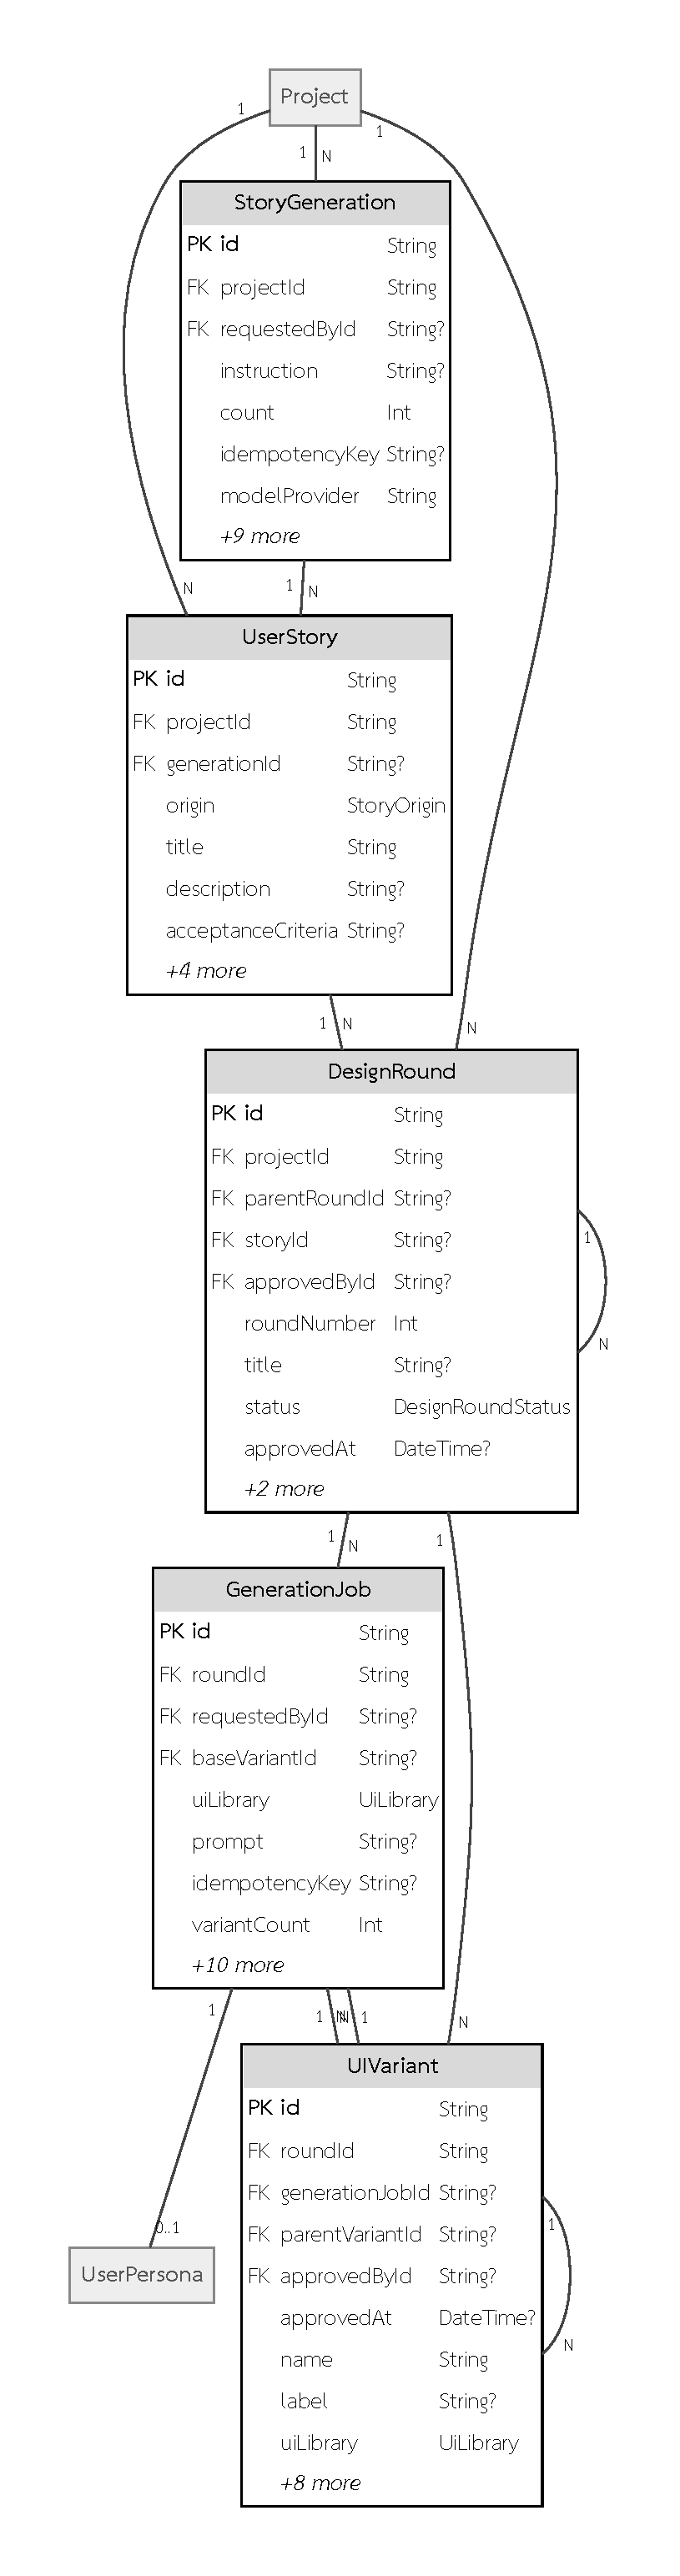
\includegraphics[width=\linewidth,height=0.88\textheight,keepaspectratio]{figures/ch3-methodology/er-design-generation.pdf}
  \caption{ER diagram ส่วนการออกแบบและการสร้าง UI ด้วย AI}
  \label{fig:er-design-generation}
\end{figure}
\begin{figure}[p]
  \centering
  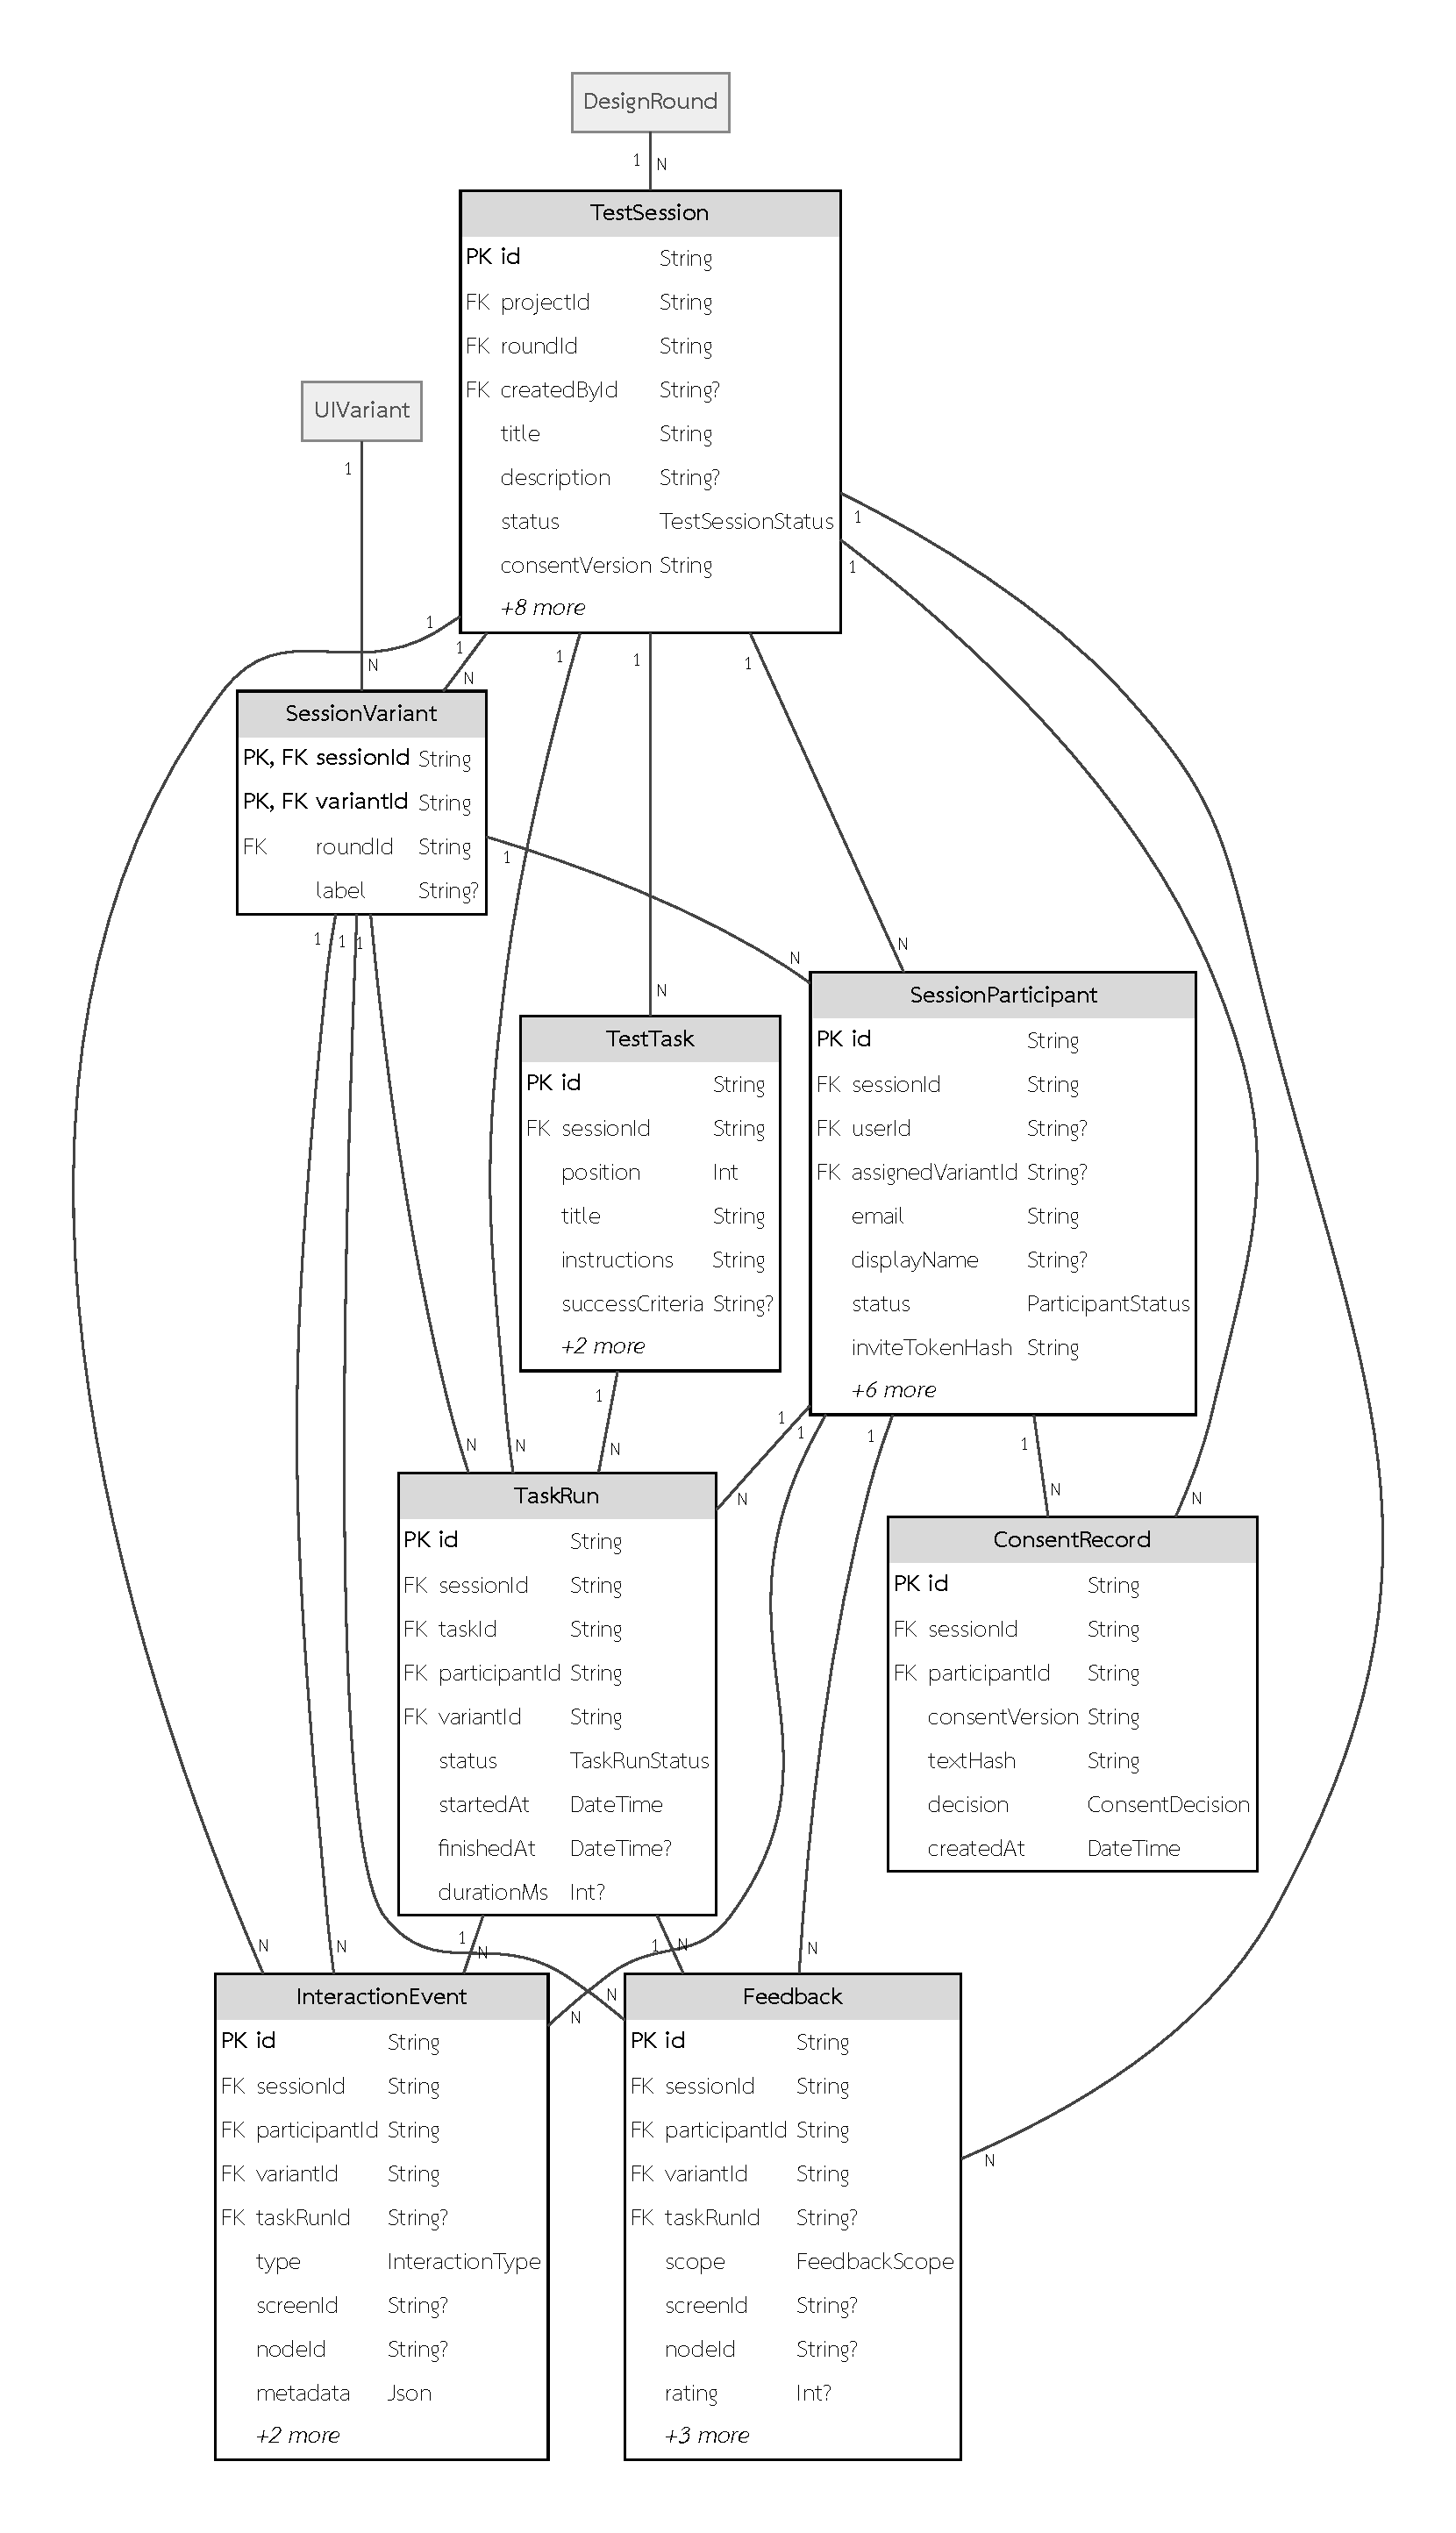
\includegraphics[width=\linewidth,height=0.88\textheight,keepaspectratio]{figures/ch3-methodology/er-testing.pdf}
  \caption{ER diagram ส่วนเซสชันการทดสอบ}
  \label{fig:er-testing}
\end{figure}
\begin{figure}[p]
  \centering
  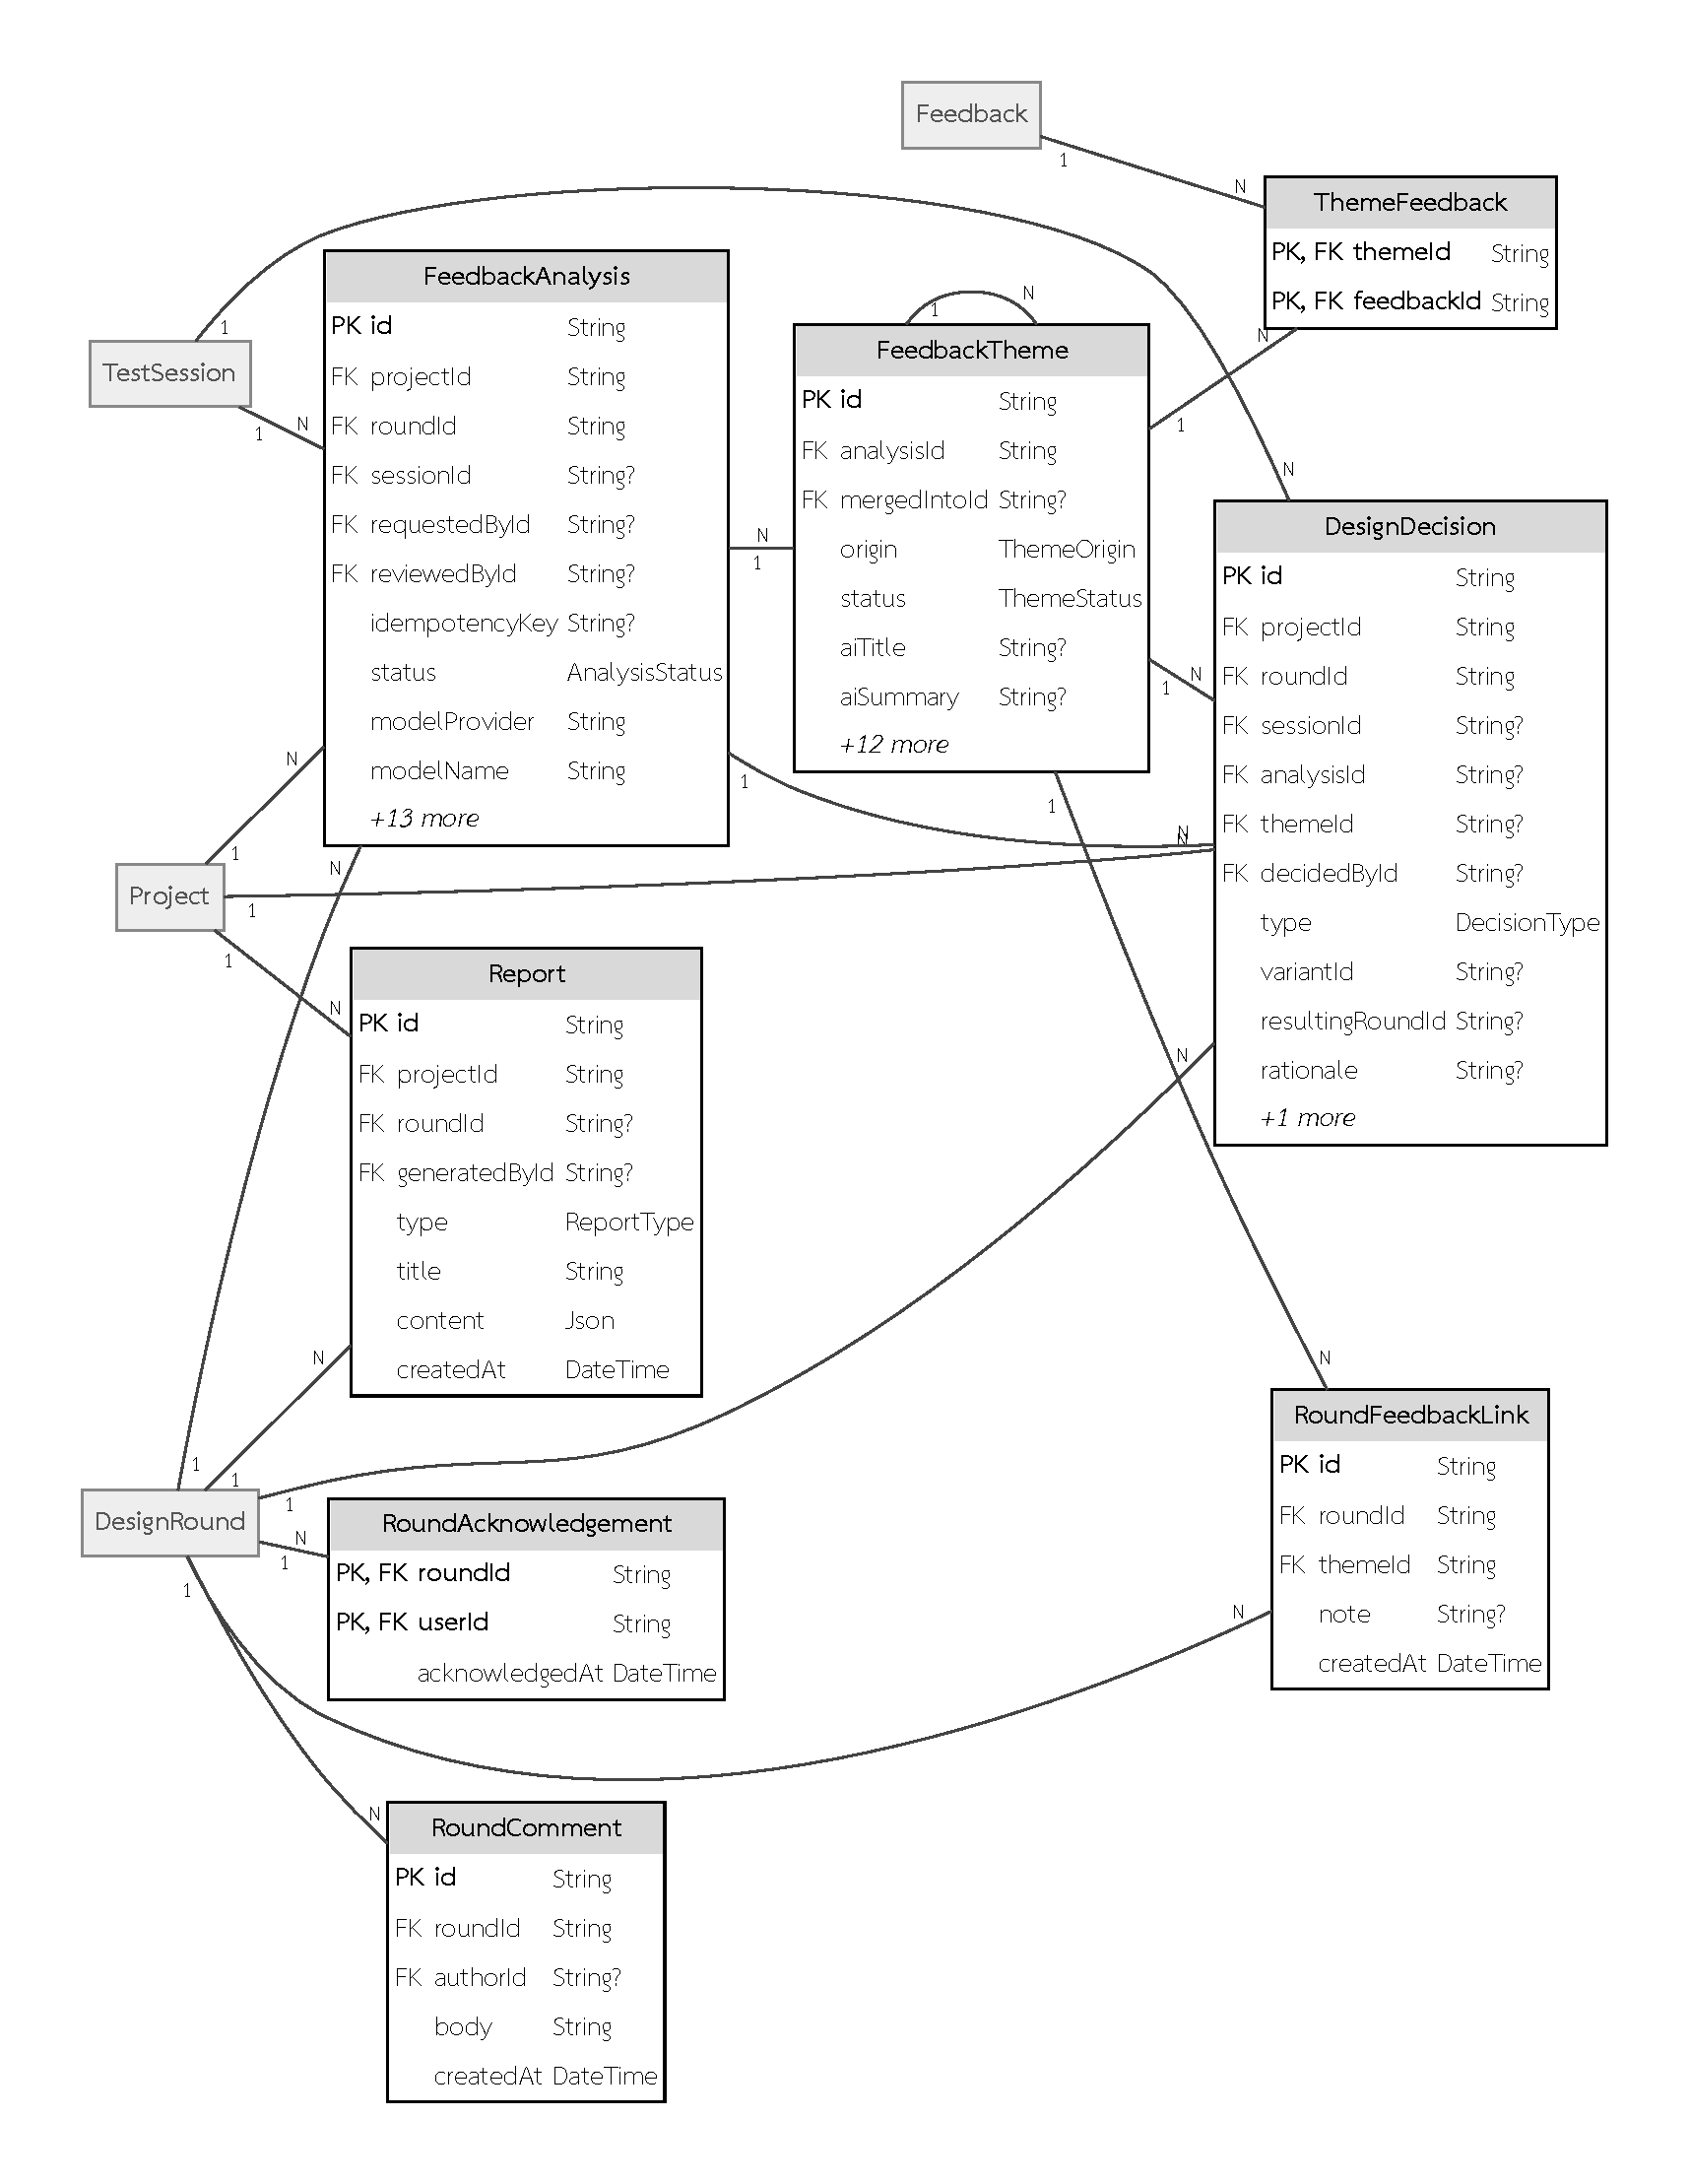
\includegraphics[width=\linewidth,height=0.88\textheight,keepaspectratio]{figures/ch3-methodology/er-analysis-report.pdf}
  \caption{ER diagram ส่วนการวิเคราะห์ข้อเสนอแนะและรายงาน}
  \label{fig:er-analysis-report}
\end{figure}

\subsection{User Flow และแผนผังเว็บไซต์ (Site Map)}
\thaijustify{
  \todo{User flow และ sitemap ให้ตรงกับ hi-fi v2}
}


\section{สถาปัตยกรรมโดยภาพรวมของระบบ}
\begin{figure}[H]
  \centering
  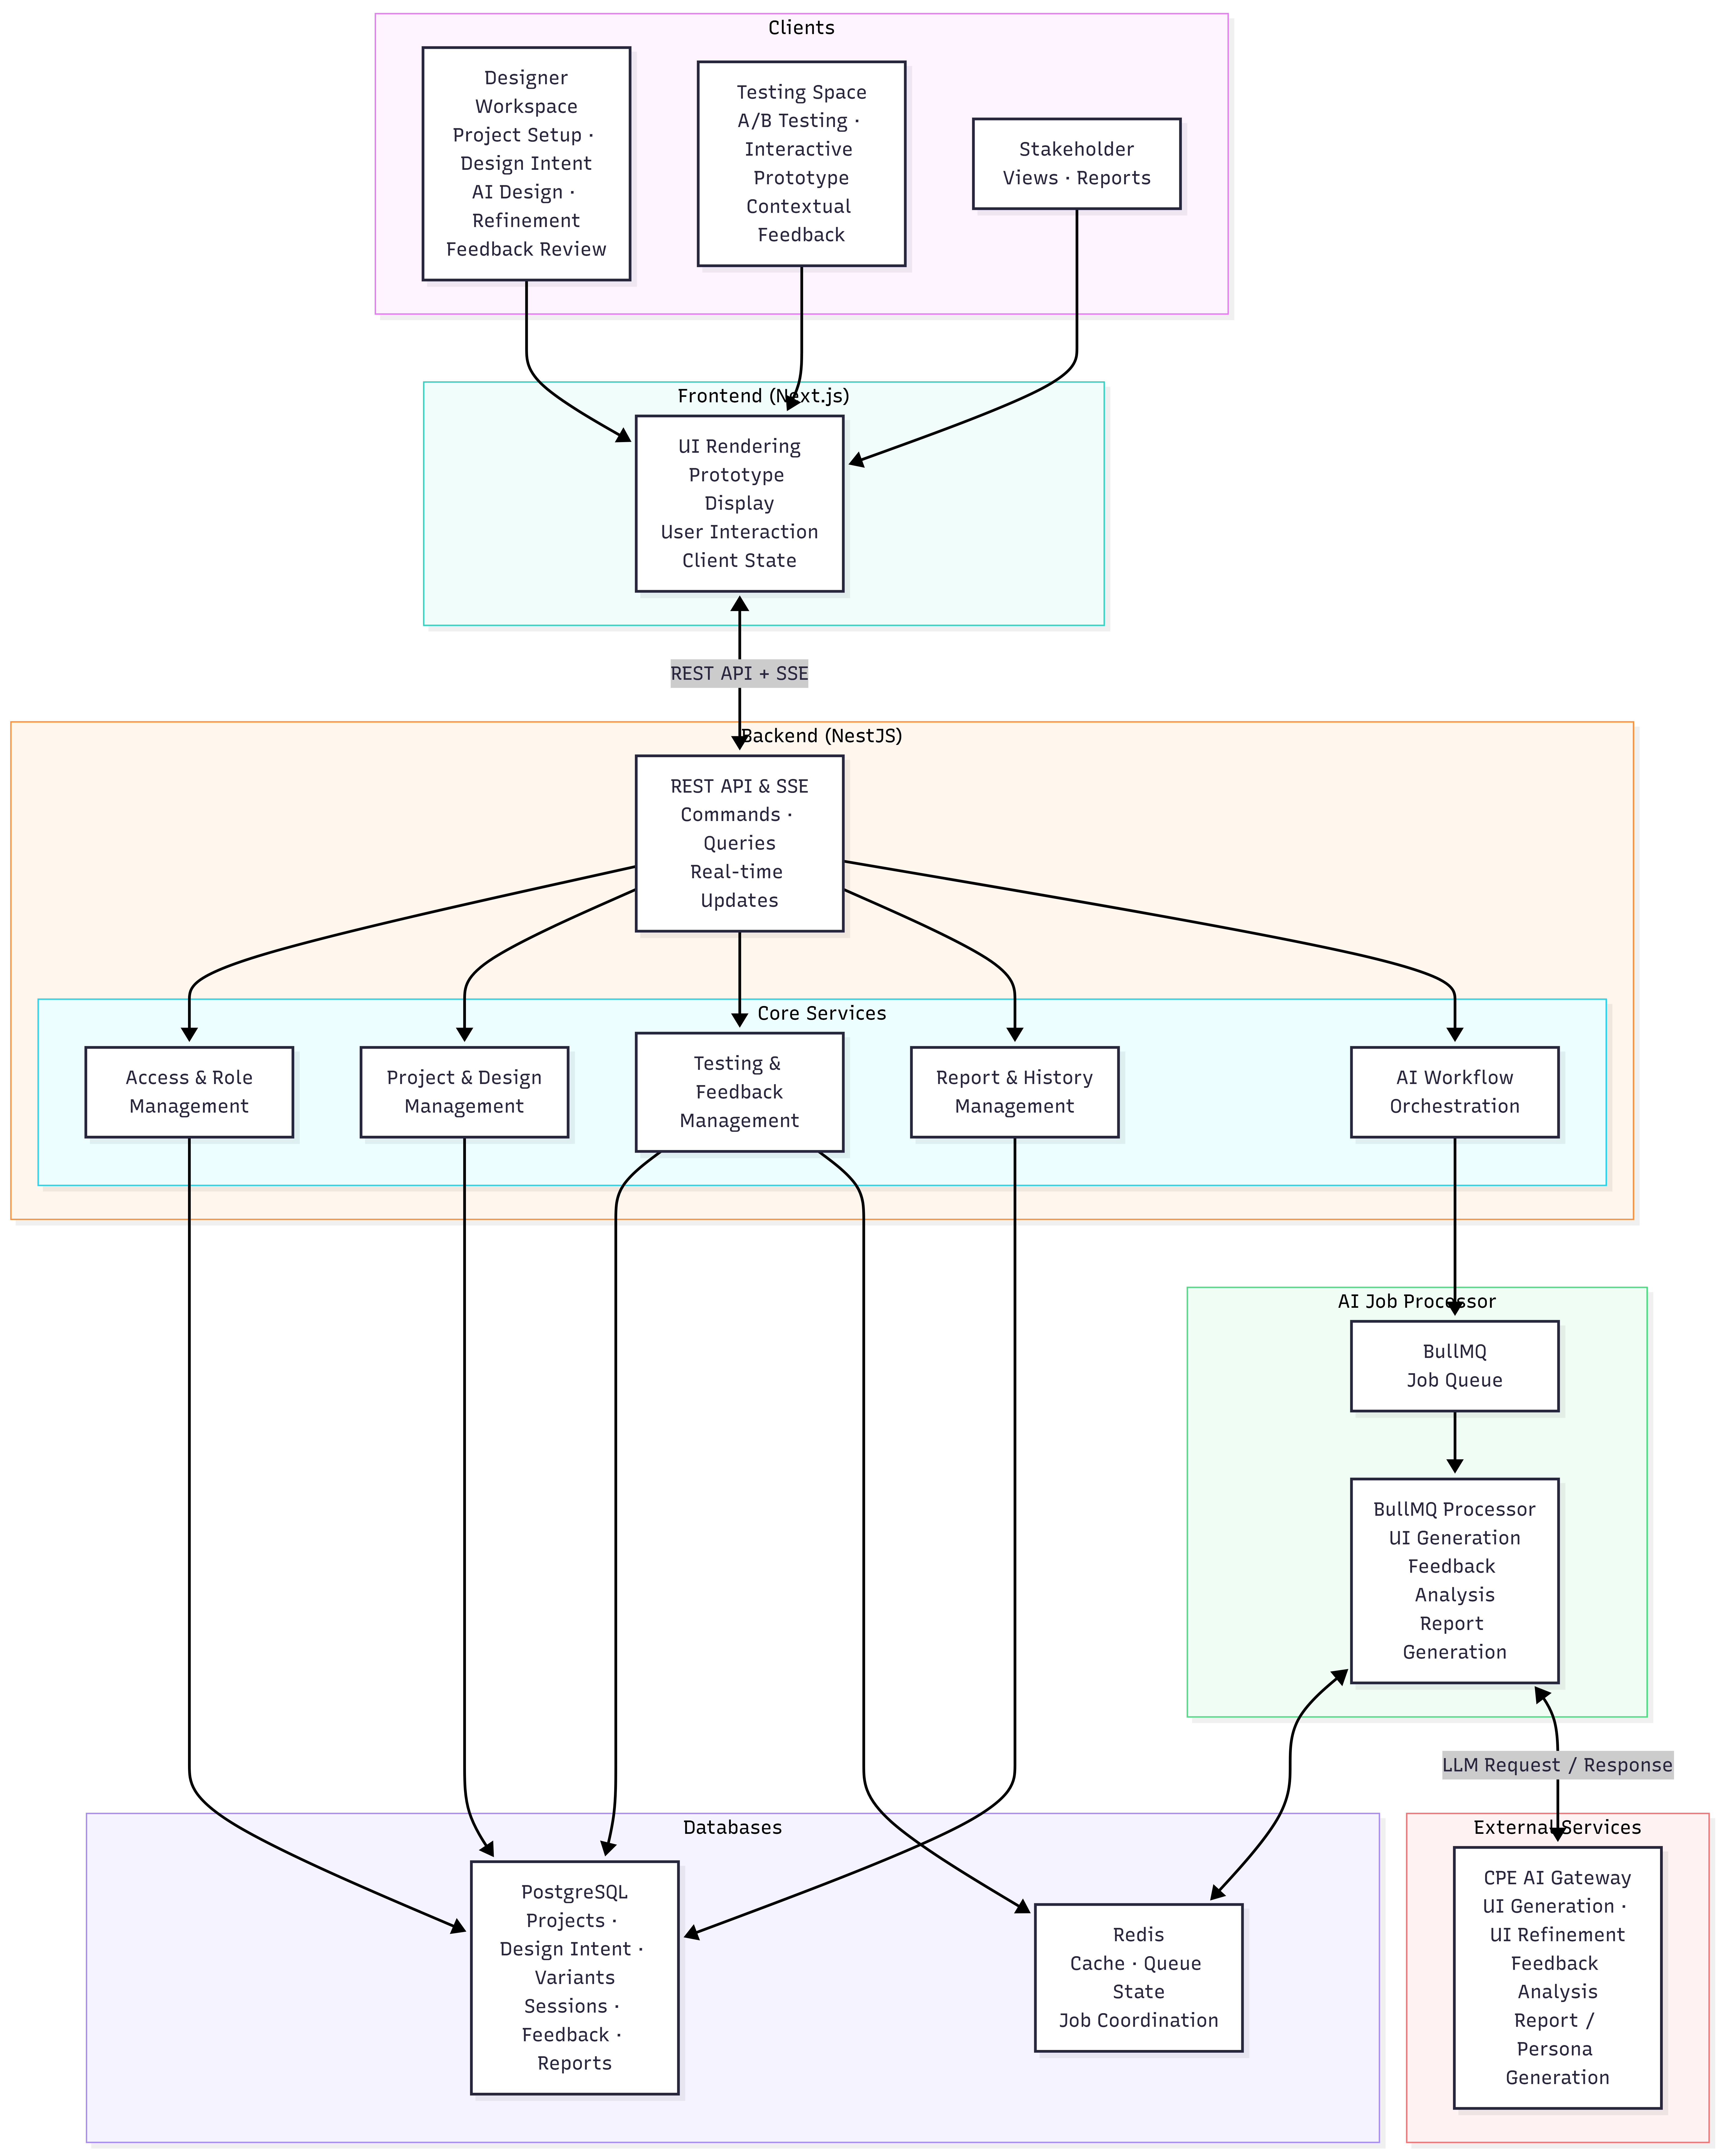
\includegraphics[
    width=0.8\linewidth,
    height=\textheight,
    keepaspectratio
  ]{figures/ch3-methodology/sys-arch3.png}
  \caption{System architecture}
  \label{fig:tech-stack-system-architecture}
  \thaijustify{ภาพแสดงสถาปัตยกรรมระบบโดยแบ่งออกเป็น Client, Frontend, Backend, AI Job Processor, Database และ External Services โดย Frontend พัฒนาด้วย Next.js และสื่อสารกับ Backend ผ่าน REST API และ SSE (Server-Sent Events) ซึ่งช่วยให้ Server สามารถส่งข้อมูลและการอัปเดตแบบ Real-time ไปยัง Client ได้โดยไม่ต้องส่ง Request ใหม่ ขณะที่ Backend ซึ่งพัฒนาด้วย NestJS ทำหน้าที่จัดการสิทธิ์ ข้อมูลโครงการ การทดสอบ Feedback รายงาน และกระบวนการ AI โดยงานที่ต้องใช้เวลาประมวลผลจะถูกส่งผ่าน BullMQ ไปยัง AI Job Processor และเชื่อมต่อกับ CPE AI Gateway สำหรับการประมวลผลด้วย AI}
\end{figure}

\subsection{เทคโนโลยีที่ใช้ในแต่ละส่วน}
\thaijustify{
  ซอร์สโค้ดทั้งหมดจัดเก็บใน repository เดียวแบบ monorepo จัดการด้วย Turborepo และ pnpm แบ่งเป็นสองแอปพลิเคชัน คือ frontend และ backend เทคโนโลยีที่ใช้ในแต่ละส่วนแสดงในตารางที่~\ref{tab:tech-stack}
}
\begin{table}[H]
  \centering
  \caption{เทคโนโลยีที่ใช้ในแต่ละส่วนของระบบ}
  \label{tab:tech-stack}
  \small
  \begin{tabularx}{\linewidth}{|>{\RaggedRight\arraybackslash}p{0.2\linewidth}|>{\RaggedRight\arraybackslash}p{0.3\linewidth}|>{\RaggedRight\arraybackslash}X|}
    \hline
    \textbf{ส่วนของระบบ} & \textbf{เทคโนโลยี} & \textbf{หน้าที่} \\ \hline
    Frontend & Next.js 16, React 19, TypeScript & หน้าจอของผู้ใช้ทุกบทบาท \\ \hline
    UI library & shadcn/ui (Radix UI), Tailwind CSS, Hugeicons & component และไอคอนตาม design system ของแพลตฟอร์ม \\ \hline
    Backend & NestJS 11, TypeScript & REST API, การยืนยันตัวตน, การควบคุมสิทธิ์ และงาน AI \\ \hline
    ฐานข้อมูล & PostgreSQL 17, Prisma 7 & จัดเก็บข้อมูลทั้งหมด และจัดการ migration ของ schema \\ \hline
    Cache และคิวงาน & Redis 7, BullMQ & cache ของ response และคิวงานที่ใช้เวลานาน เช่น การสร้าง UI \\ \hline
    การสื่อสารแบบ real-time & Server-Sent Events (SSE) & ส่งความคืบหน้าและความคิดของโมเดลระหว่างประมวลผลไปยังหน้าจอ \\ \hline
    การยืนยันตัวตน & Passport (Google OAuth 2.0), JWT & เข้าสู่ระบบและออก access token กับ refresh token \\ \hline
    บริการ AI & CPE AI Gateway (API แบบเดียวกับ OpenAI) & muse-glimmer-30b สร้าง UI และ qwen3.8-27b วิเคราะห์ข้อเสนอแนะ ร่าง user story, prompt และ persona \\ \hline
    เอกสาร API & Swagger (OpenAPI) & เอกสารและเครื่องมือทดลองเรียก API \\ \hline
    การทดสอบ & Jest & unit test และ end-to-end test ของ backend \\ \hline
    CI & GitHub Actions & ตรวจชื่อ pull request, lint และ build ทุก pull request \\ \hline
  \end{tabularx}
\end{table}

\section{การออกแบบ User Interface Prototype}
\thaijustify{
  \todo{Design system และหน้าจอ hi-fi จาก Figma พร้อมคำอธิบาย}
}

\section{การพัฒนาระบบ}
\thaijustify{
  ในภาคการศึกษาที่ 1 การพัฒนาระบบดำเนินการตาม milestone M0 ถึง M3 โดยใช้ GitHub เป็นที่เก็บซอร์สโค้ด ทุกการเปลี่ยนแปลงผ่าน pull request และตั้งชื่อตามรูปแบบ conventional commit จนถึงวันที่ 26 พฤศจิกายน 2569 มีการ commit ทั้งหมด 178 ครั้ง รายละเอียดของแต่ละ milestone มีดังนี้
}

\subsection{M0: Foundation}
\thaijustify{
  ช่วง Foundation เป็นการวางโครงสร้างพื้นฐานของโปรเจกต์ ได้แก่
  \begin{itemize}
    \item \textbf{โครงสร้างซอร์สโค้ด:} monorepo ที่มี frontend และ backend ใช้คำสั่งเดียวในการรัน build, lint และ test ทั้งระบบ
    \item \textbf{สภาพแวดล้อมสำหรับพัฒนา:} ใช้ Docker Compose รัน PostgreSQL และ Redis มีสคริปต์สร้างไฟล์ตั้งค่า สร้างผู้ใช้ทดสอบ และออก token สำหรับทดสอบ API โดยไม่ต้องเข้าสู่ระบบผ่าน Google
    \item \textbf{Data model:} ออกแบบ schema ของฐานข้อมูลครอบคลุมทุก milestone ตั้งแต่ผู้ใช้จนถึงรายงาน (หัวข้อ~\ref{sec:er-diagram}) และจัดการการเปลี่ยนแปลงด้วย migration ซึ่งมีทั้งหมด 7 ชุด โดยกำหนดให้ migration ที่ merge แล้วแก้ไขไม่ได้ เพื่อให้ฐานข้อมูลของทุกคนตรงกัน
    \item \textbf{Design system:} ใช้ shadcn/ui เป็นพื้นฐานของหน้าจอแพลตฟอร์ม และเตรียม UI kit สองชุด คือ shadcn/ui และ MUI ให้ AI ใช้สร้างหน้าจอตามที่นักออกแบบเลือก
    \item \textbf{PDPA:} ออกแบบการเก็บความยินยอมของผู้เข้าร่วมทดสอบพร้อมเวอร์ชันของข้อความ เพื่อใช้ใน M4
    \item \textbf{CI:} GitHub Actions ตรวจทุก pull request โดยเรียงเป็นสามขั้น คือ ชื่อ pull request, lint และ build
  \end{itemize}
  ส่วนที่ยังไม่ได้ทำคือการ deploy อัตโนมัติ (CD) และระบบเก็บ event analytics
}

\subsection{M1: Secure Access}
\thaijustify{
  ระบบยืนยันตัวตนปัจจุบันใช้การเข้าสู่ระบบด้วยบัญชี Google ผ่าน OAuth 2.0 เมื่อเข้าสู่ระบบสำเร็จ backend ออก access token แบบ JWT ที่มีอายุ 15 นาที และ refresh token ที่มีอายุ 30 วัน refresh token ถูกเก็บเป็นค่า hash และเปลี่ยนใหม่ทุกครั้งที่ใช้ (token rotation) หากมีการนำ token ที่ถูกใช้ไปแล้วกลับมาใช้ซ้ำ ระบบจะถือว่า token รั่วไหลและยกเลิก token ทั้งกลุ่มของการเข้าสู่ระบบนั้น
}
\thaijustify{
  การควบคุมสิทธิ์ใช้แนวทาง permission-based access control กล่าวคือ แต่ละบทบาทในโปรเจกต์ (Designer, Project Manager, Client และ Developer) ได้รับชุดสิทธิ์ เช่น \texttt{design:write}, \texttt{design:approve} และ \texttt{handoff:read} และ API แต่ละเส้นตรวจเฉพาะสิทธิ์ที่ต้องใช้ ไม่ได้ตรวจชื่อบทบาทโดยตรง ทำให้ปรับสิทธิ์ของแต่ละบทบาทได้ในที่เดียว นอกจากนี้ระบบบันทึกการกระทำสำคัญลง audit log และมี end-to-end test ตรวจการควบคุมสิทธิ์
}
\thaijustify{
  หน้าจอสมัครสมาชิก เข้าสู่ระบบ และลืมรหัสผ่านพัฒนาส่วน frontend แล้ว ส่วนการสมัครด้วยอีเมลและรหัสผ่าน การยืนยันอีเมล และการรีเซ็ตรหัสผ่านฝั่ง backend อยู่ระหว่างพัฒนาใน branch แยก และจะรวมเข้า branch หลักภายในภาคการศึกษาที่ 1
}
\todo{ภาพหน้าจอเข้าสู่ระบบและสมัครสมาชิก}

\subsection{M2: Project Setup}
\thaijustify{
  ผู้ใช้สร้าง workspace ตั้งรูปประจำ workspace และเชิญสมาชิกด้วยอีเมลได้ ภายใน workspace นักออกแบบสร้างโปรเจกต์ กำหนดสมาชิกและบทบาทในโปรเจกต์ และค้นหาหรือกรองโปรเจกต์ได้ทั้งแบบรายการและแบบแกลเลอรี
}
\thaijustify{
  ความต้องการทางการออกแบบ (design intent) ของโปรเจกต์ประกอบด้วยเป้าหมายของการออกแบบ design system ที่เลือก (shadcn/ui หรือ MUI) มาตรฐานการเข้าถึง (ค่าเริ่มต้น WCAG 2.1 AA) แนวทางการออกแบบ สีแบรนด์สามสี แนวทาง CI และ tone of voice ทุกครั้งที่แก้ไข ระบบจะเพิ่มเลขเวอร์ชันของ design intent และงานสร้าง UI แต่ละครั้งเก็บสำเนาของ design intent ที่ใช้ไว้ ทำให้ design intent เป็น context ที่ AI นำไปใช้ซ้ำได้ และตรวจสอบย้อนหลังได้ว่า UI แต่ละชุดสร้างจาก design intent ฉบับใด นอกจากนี้นักออกแบบเพิ่ม persona ของผู้ใช้เป้าหมายเองได้ และหน้าภาพรวมของโปรเจกต์แสดงกิจกรรมล่าสุดจาก audit log
}
\todo{ภาพหน้าจอสร้างโปรเจกต์และหน้าจอ design intent}

\subsection{M3: AI Design Generation}
\thaijustify{
  นักออกแบบเขียน user story และ problem statement ผ่านหน้าจอ ซึ่ง backend รองรับการให้ AI ร่าง user story แล้วแต่ยังไม่มีหน้าจอสำหรับส่วนนี้ จากนั้น AI ร่าง structured prompt จาก design intent, persona และ user story และส่งผลลัพธ์พร้อมความคิดของโมเดลมาแสดงแบบ real-time ผ่าน SSE นักออกแบบเลือก persona ตรวจ และแก้ prompt ก่อนสั่งสร้าง UI
}
\thaijustify{
  การสร้าง UI เป็นไปตามขั้นตอนในรูปที่~\ref{fig:generation-pipeline} ระบบสร้าง persona artifact จาก prompt ก่อน (ข้ามขั้นนี้ได้หากนักออกแบบเลือก persona ไว้แล้ว) จากนั้นสร้างหน้าจอแบบ high-fidelity เป็น HTML ทีละ variant ค่าเริ่มต้นคือสอง variant (A และ B) สำหรับ comparative usability testing HTML ที่ได้จะถูก sanitize และตรวจโครงสร้าง การใช้ component ของ UI kit สีแบรนด์ platform และการเข้าถึงตามมาตรฐานใน design intent หากไม่ผ่าน ระบบส่งปัญหาที่พบกลับให้โมเดลแก้ได้สูงสุดสองครั้ง ระหว่างนั้นหน้าจอแสดงความคิดของโมเดลและสถานะของแต่ละขั้นแบบ real-time (generation trace) และนักออกแบบยกเลิกงานได้
}
\begin{figure}[H]
  \centering
  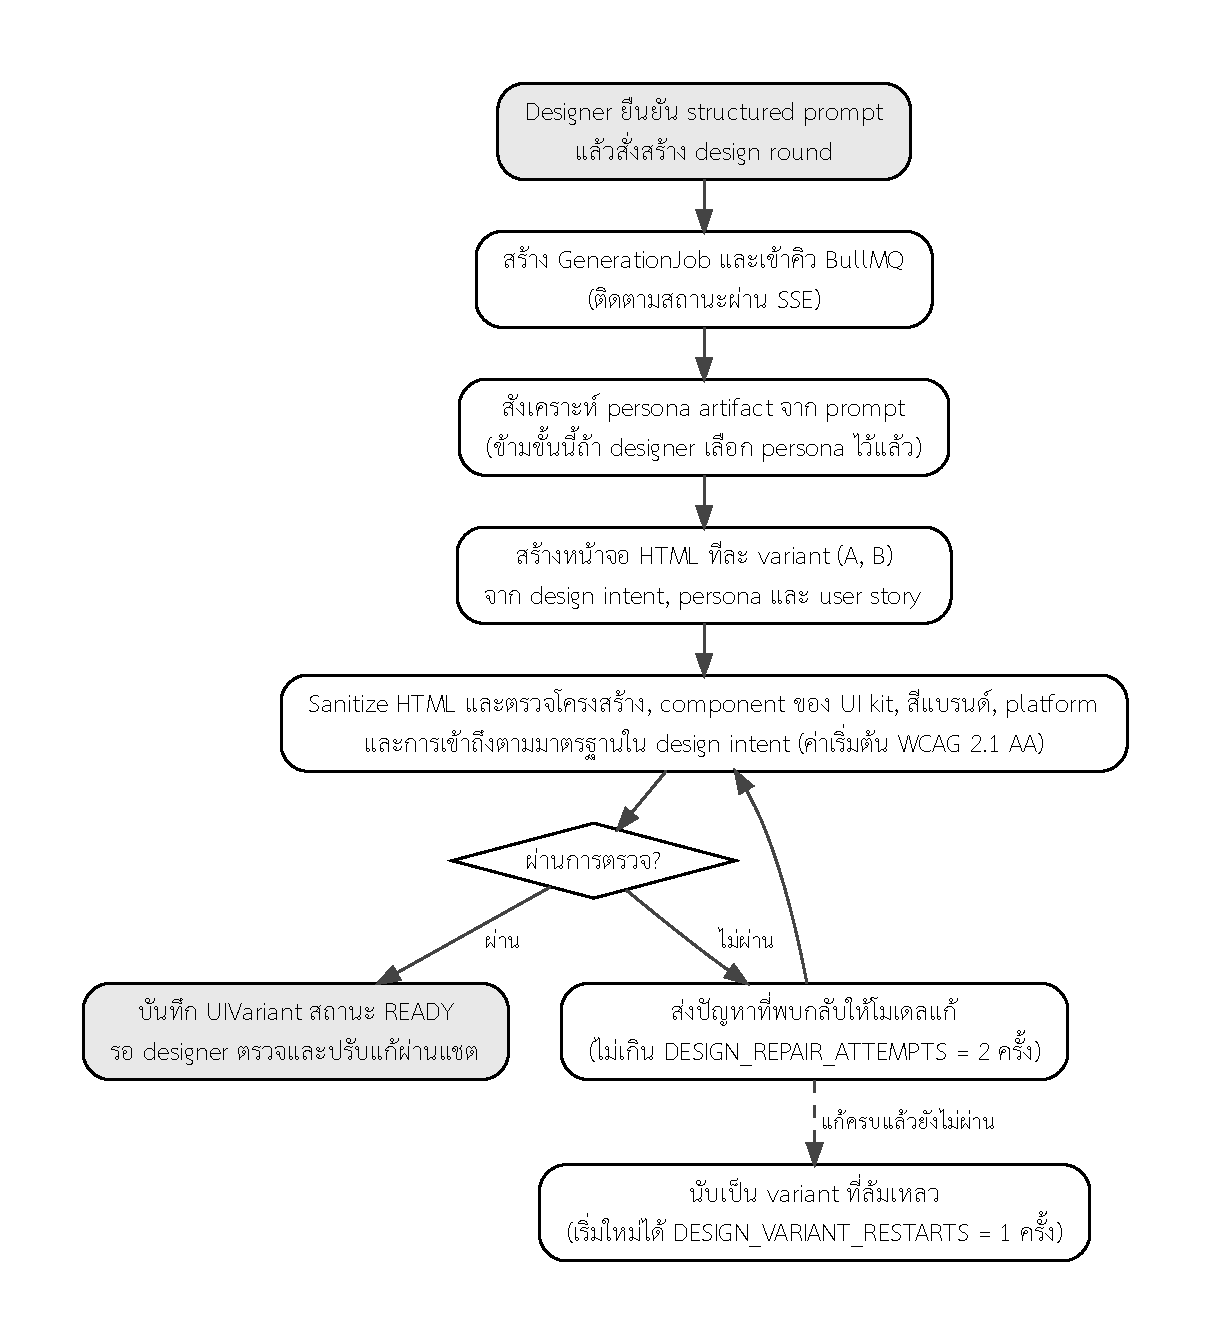
\includegraphics[width=0.78\linewidth]{figures/ch3-methodology/generation-pipeline.pdf}
  \caption{ขั้นตอนการสร้าง UI variant ด้วย AI}
  \label{fig:generation-pipeline}
\end{figure}
\thaijustify{
  หลังได้ variant แล้ว นักออกแบบดูตัวอย่างหน้าจอและปรับแก้ผ่านแชต (chat-based refinement) การแก้แต่ละครั้งสร้าง variant เวอร์ชันใหม่ที่อ้างอิงฉบับเดิม จึงย้อนดูเวอร์ชันก่อนหน้าได้ เมื่อพอใจแล้วนักออกแบบอนุมัติ variant เพื่อนำไปทดสอบ สำหรับการกำหนดภารกิจและการเริ่มเซสชันการทดสอบ backend รองรับแล้ว แต่หน้าจอฝั่ง frontend อยู่ในแผนของภาคการศึกษาที่ 2
}
\todo{ภาพหน้าจอ user story, การตรวจ prompt, generation trace และการปรับแก้ผ่านแชต}

\subsection{Application Program Interface}
\thaijustify{
  Backend ให้บริการผ่าน REST API ที่มีเอกสารแบบ OpenAPI ผ่าน Swagger UI API ส่วนใหญ่ต้องใช้ access token ของผู้ใช้ ส่วน API ของผู้เข้าร่วมทดสอบใช้ token ที่แลกได้จากลิงก์เชิญ ซึ่งมีอายุไม่เกินระยะเวลาของเซสชัน งานที่ใช้เวลานานมี endpoint แบบ SSE สำหรับติดตามความคืบหน้า กลุ่มของ API แสดงในตารางที่~\ref{tab:api-groups}
}
\begingroup
\small
\begin{xltabular}{\linewidth}{|>{\RaggedRight\arraybackslash}p{0.36\linewidth}|>{\RaggedRight\arraybackslash}X|}
  \caption{กลุ่มของ API ในระบบ}\label{tab:api-groups}\\
  \hline
  \textbf{Path} & \textbf{หน้าที่} \\ \hline
  \endfirsthead
  \hline
  \textbf{Path} & \textbf{หน้าที่} \\ \hline
  \endhead
  \texttt{/auth} & เข้าสู่ระบบด้วย Google, ขอ token ใหม่ และออกจากระบบ \\ \hline
  \texttt{/users} & ข้อมูลและรูปโปรไฟล์ของผู้ใช้ \\ \hline
  \texttt{/workspaces} & จัดการ workspace, สมาชิก, คำเชิญ และรูปประจำ workspace \\ \hline
  \texttt{/projects}, \texttt{/projects/:id/members} & จัดการโปรเจกต์และสมาชิกในโปรเจกต์ \\ \hline
  \texttt{/projects/:id/design-intent}, \texttt{personas}, \texttt{user-stories} & ความต้องการทางการออกแบบ, persona และ user story \\ \hline
  \texttt{/projects/:id/story-generations} & ให้ AI ร่าง user story (มี SSE) \\ \hline
  \texttt{/projects/:id/rounds} & รอบการออกแบบ, การร่าง prompt (SSE) และการอนุมัติรอบ \\ \hline
  \texttt{/projects/:id/rounds/:id/generation-jobs} & สั่ง ติดตาม (SSE) และยกเลิกงานสร้าง UI \\ \hline
  \texttt{/projects/:id/variants} & ดู ปรับแก้ อนุมัติ และดูประวัติเวอร์ชันของ variant \\ \hline
  \texttt{/projects/:id/test-sessions} & เซสชันการทดสอบ ภารกิจ ผู้เข้าร่วม และผลการทดสอบ \\ \hline
  \texttt{/testing} & API ของผู้เข้าร่วมทดสอบ: เข้าร่วม, ให้ความยินยอม, ทำภารกิจ, ส่งพฤติกรรมและข้อเสนอแนะ \\ \hline
  \texttt{/projects/:id/analyses}, \texttt{themes} & วิเคราะห์ข้อเสนอแนะด้วย AI และจัดการประเด็น \\ \hline
  \texttt{/projects/:id/rounds/:id/iterate}, \texttt{decisions} & เริ่มรอบถัดไปจากประเด็นที่เลือก และประวัติการตัดสินใจ \\ \hline
  \texttt{/projects/:id/shared-rounds}, \texttt{handoff}, \texttt{status}, \texttt{reports} & มุมมองและรายงานของ Client, Developer และ Project Manager \\ \hline
  \texttt{/projects/:id/audit-logs}, \texttt{/health} & บันทึกกิจกรรม และตรวจสถานะระบบ \\ \hline
\end{xltabular}
\endgroup
\thaijustify{
  API กลุ่มเซสชันการทดสอบ การวิเคราะห์ข้อเสนอแนะ และรายงาน พัฒนาส่วน backend ไว้ล่วงหน้าแล้ว ส่วนหน้าจอที่ใช้ API เหล่านี้อยู่ในแผนของภาคการศึกษาที่ 2
}
\todo{ภาพหน้าจอ Swagger UI}
